% CoRL 2026 Submission
\documentclass[conference]{IEEEtran}
\usepackage{amsmath,amssymb,amsfonts}
\usepackage{graphicx}
\usepackage{textcomp}
\usepackage{xcolor}
\usepackage{url}
\usepackage{booktabs}
\usepackage{multirow}
\usepackage{subcaption}
\usepackage{tikz}
\usetikzlibrary{shapes.geometric,arrows.meta,positioning,fit,calc}
\usepackage{placeins}
\usepackage{caption}
\usepackage[hidelinks]{hyperref}

% Tighten figure/table spacing to avoid overflow and orphan captions
\captionsetup{font=small,labelfont=bf,skip=4pt,justification=raggedright,singlelinecheck=false}
\captionsetup[subfigure]{font=footnotesize,labelfont=bf,skip=2pt,justification=raggedright,singlelinecheck=false}
\setlength{\textfloatsep}{8pt plus 1.0pt minus 2.0pt}
\setlength{\floatsep}{6pt plus 1.0pt minus 2.0pt}
\setlength{\intextsep}{6pt plus 1.0pt minus 2.0pt}
\setlength{\abovecaptionskip}{4pt}
\setlength{\belowcaptionskip}{0pt}

\newcommand{\brier}{B_{\mathrm{soft}}}
\newcommand{\kl}{D_{\mathrm{KL}}}
\newcommand{\hmax}{H_{\max}}

\begin{document}

\title{Human-Aligned Sidewalk Accessibility Perception: Soft-Label Learning from 829 Mobility Aid Users for Autonomous Mobility Services}

\maketitle

\begin{abstract}
Before a shared autonomous vehicle opens its door at a curbside drop-off, the planner must answer a question the on-board map almost never resolves: is the adjacent sidewalk passable for this passenger's specific mobility aid? Crowdsourced accessibility platforms capture vote distributions that prior work reduces to hard labels; we instead use the full distribution as the probabilistic training target, and frame the problem as \textbf{calibrated perception for risk-aware pedestrian routing}. Using \textbf{49{,}490 ternary votes} (yes / unsure / no) from \textbf{829 mobility-aid users} on \textbf{52 Google Street View (GSV) views} via Project Sidewalk, with $\approx 190$ judgments per (image, aid) pair across 260 pairs and ten cities, we build empirical human probability distributions over five aid types (manual wheelchair, motorized wheelchair, mobility scooter, walker, walking cane). A frozen vision encoder with a per-aid linear probe is trained via KL divergence directly against these distributions. \textbf{The headline result is calibration}: across eight encoders, 5-fold image-level cross-validation gives a soft Brier score of $0.076$ (mean over encoders) versus $0.244$ for standard cross-entropy, a $\mathbf{3.2\times}$ improvement that is robust across all eight encoders. Macro-F1 is reported as a secondary descriptor ($0.529$ Soft-KL vs.\ $0.588$ Hard-CE, mean); F1 differences are within their 95\% CIs while Brier differences are not. Walking cane (87\% positive) illustrates the failure mode of hard labels: Hard-CE achieves F1 $=0.453$, below the trivial baseline (0.467), in 6 of 8 encoders, because 5 of the 7 minority-class images have near-tied human votes; Soft-KL preserves the bimodality and recovers F1 $= 0.640$ ($+42\%$). We embed the calibrated per-aid probabilities as edge weights in a Pittsburgh pedestrian graph and show, over $10{,}000$ random OD pairs, that risk-aware Dijkstra improves mean $\hat{p}_\mathrm{yes}$ on 87.8--91.0\% of trips at 7.4--9.8\% mean distance overhead. In a 50-pair head-to-head against OpenRouteService's wheelchair profile in the same Pittsburgh graph, our method yields a higher mean $\hat{p}_\mathrm{yes}$ on every aid in this snapshot and additionally routes the $20\%$ of pairs ORS cannot reach. The intended robotics interface is explicit: this module provides a passenger-specific map prior for AV drop-off planning, to be composed with live curbside camera/LiDAR verification before committing to a stop. Throughout, results are scoped: the visual set is small (52 views), the routing graph is one city, and all routing evaluation is offline. An auxiliary encoder-transfer probe on binary curb-ramp labels in Detroit, Zurich, and Taipei is reported precisely because the Taipei result is near chance, a Western-centric-data limitation we surface rather than hide.
\end{abstract}

\begin{figure*}[!t]
\centering
\begin{subfigure}[t]{0.32\textwidth}
\centering
\vspace{0pt}
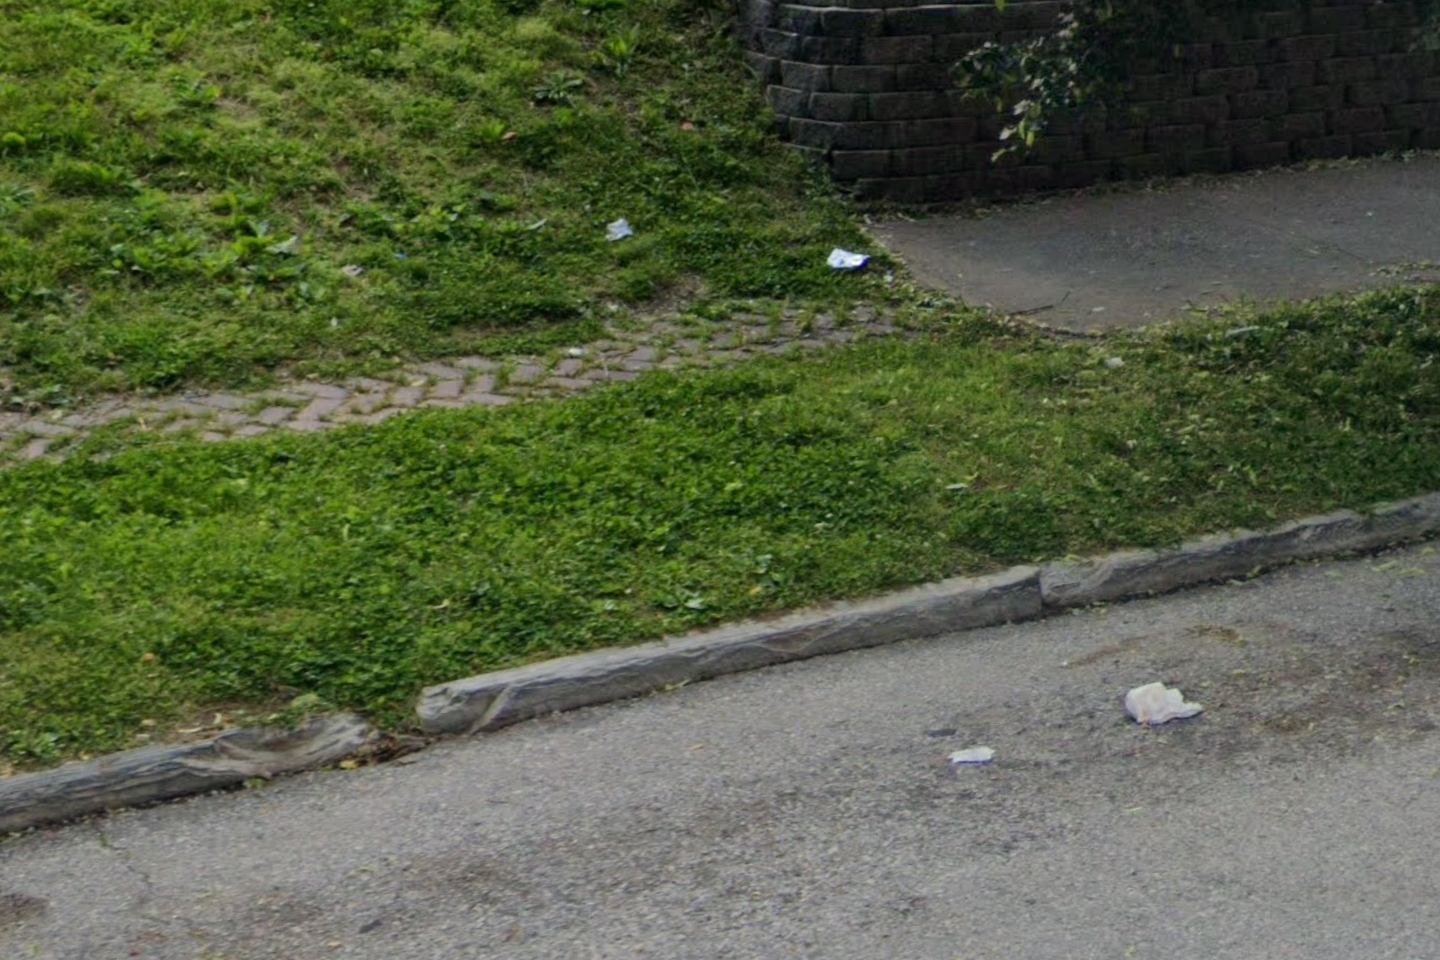
\includegraphics[width=\linewidth,height=3.0cm,keepaspectratio]{images/sidewalk.jpg}
\caption{\textbf{Divergent opinions.} Bumpy stone pavers near a curb cut produce a manual-wheelchair split of 47\%~no, 9\%~unsure, and 44\%~yes, while walking-cane users vote 76\%~yes.}
\end{subfigure}
\hfill
\begin{subfigure}[t]{0.32\textwidth}
\centering
\vspace{0pt}
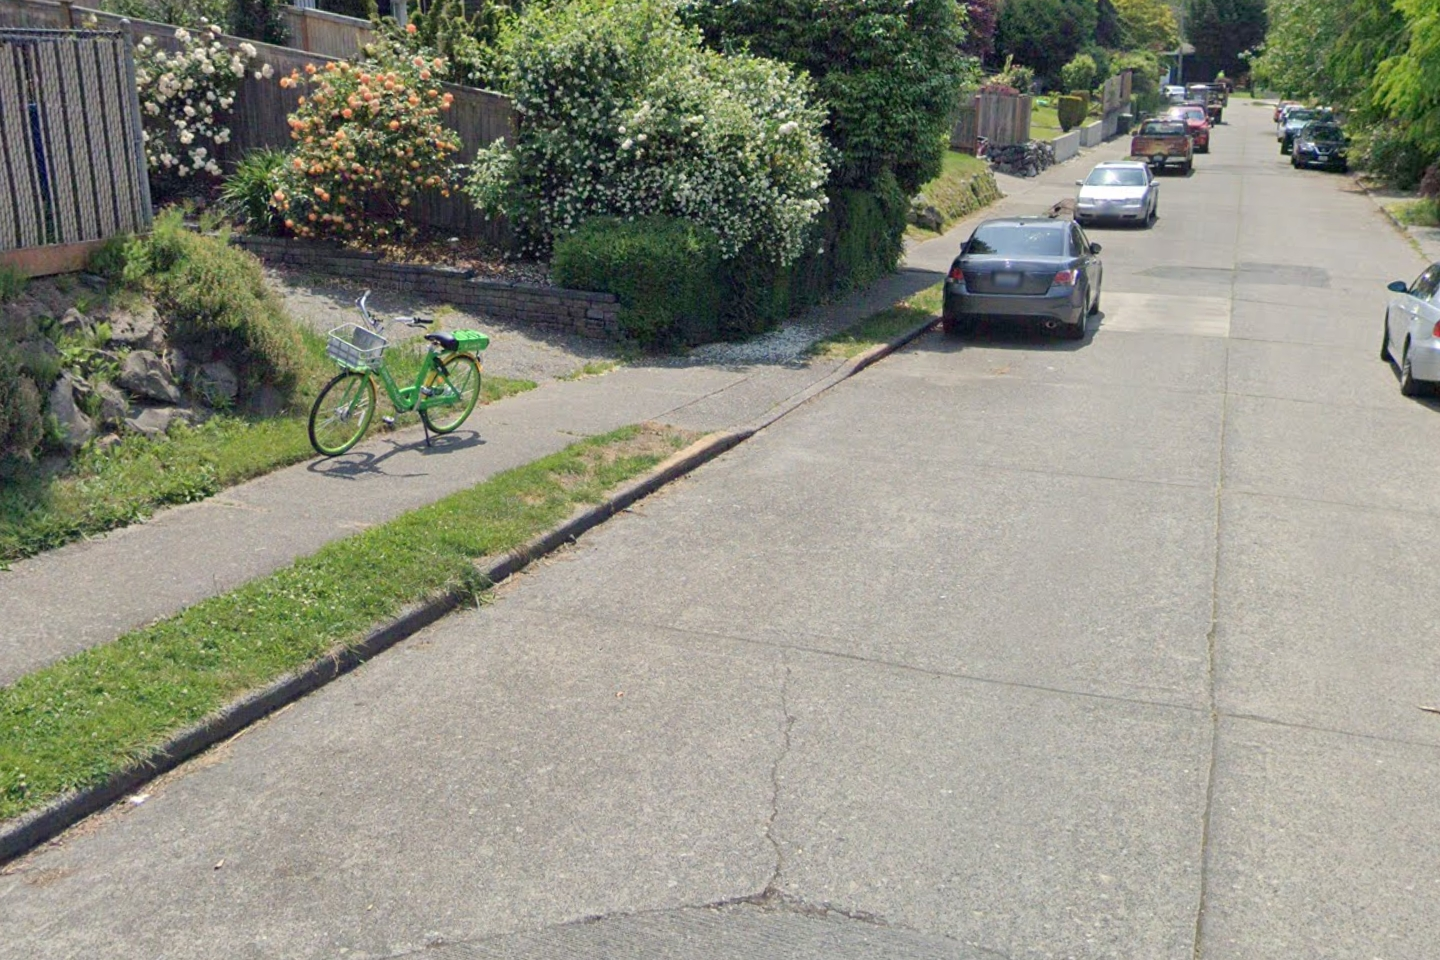
\includegraphics[width=\linewidth,height=3.0cm,keepaspectratio]{images/example2.jpg}
\caption{\textbf{Soft-label perception.} A frozen encoder plus linear probe predicts per-aid distributions $[\hat{p}_\mathrm{no}, \hat{p}_\mathrm{unsure}, \hat{p}_\mathrm{yes}]$ instead of binary classes.}
\end{subfigure}
\hfill
\begin{subfigure}[t]{0.32\textwidth}
\centering
\vspace{0pt}
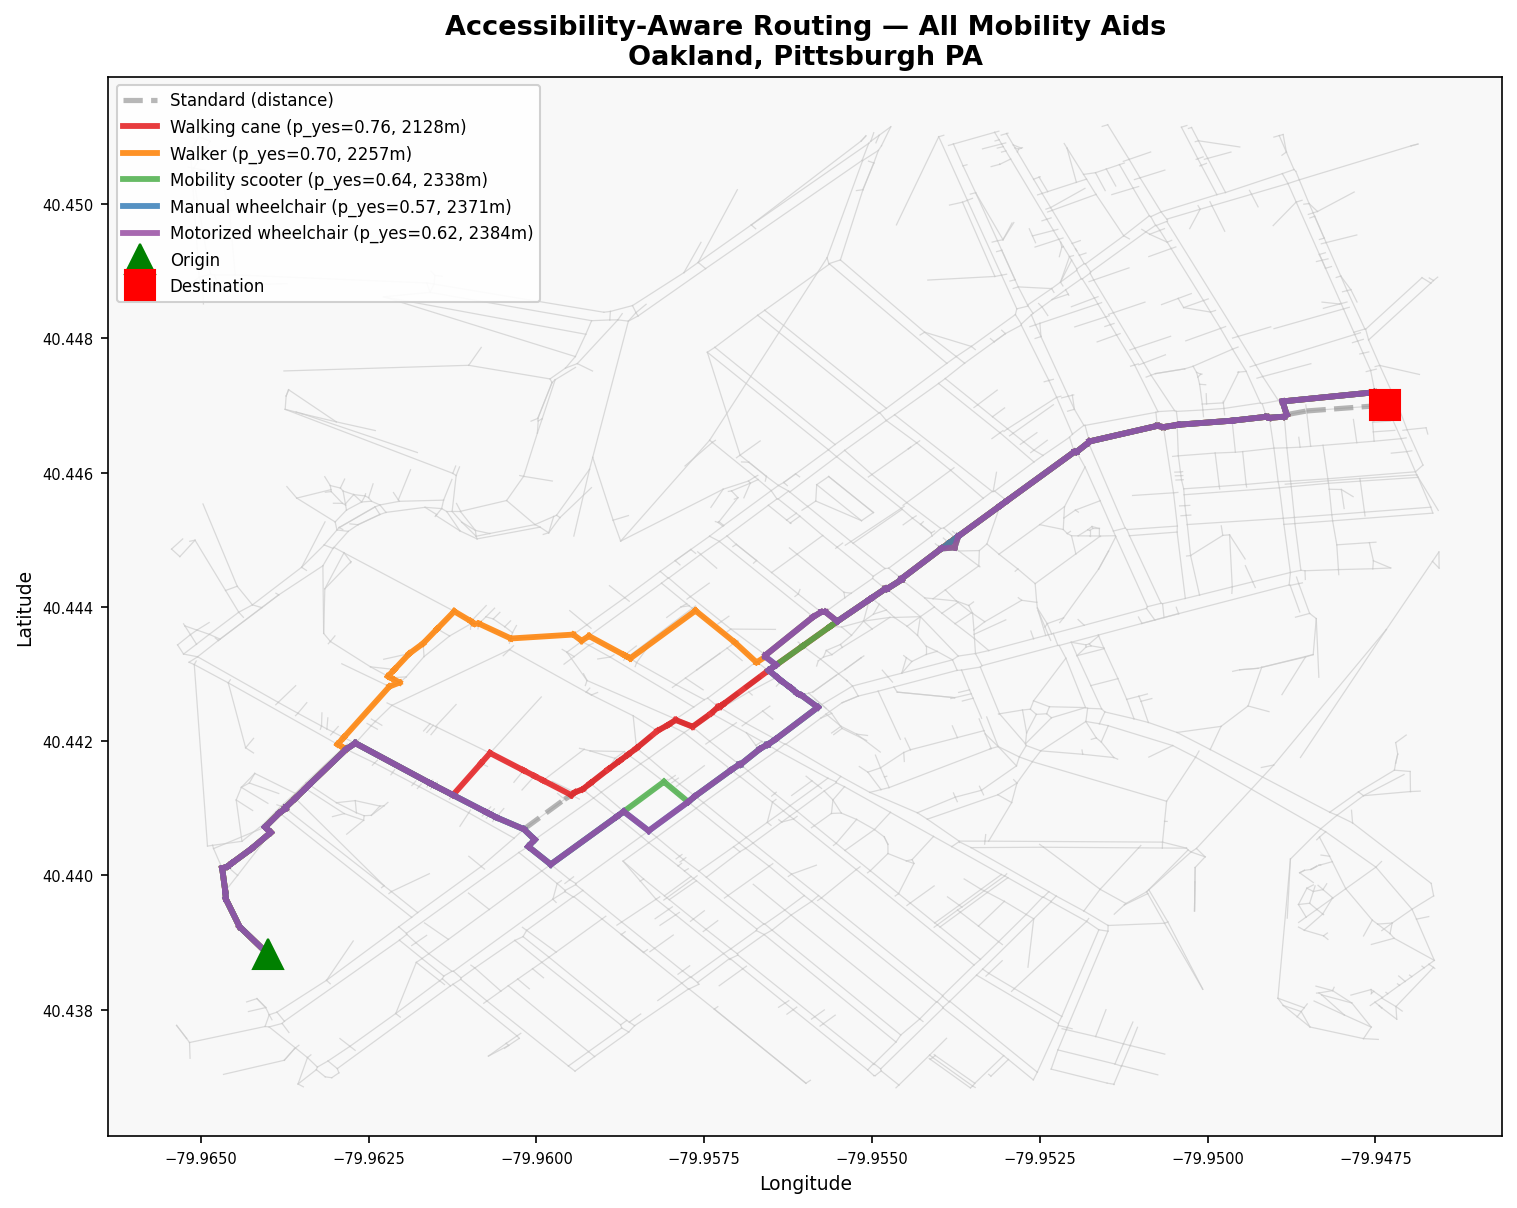
\includegraphics[width=\linewidth,height=3.0cm,keepaspectratio]{images/route_all_aids_overlay.png}
\caption{\textbf{Routing.} Calibrated per-aid edge probabilities in a Pittsburgh graph yield distinct routes per aid and beat OpenRouteService on all five aids.}
\end{subfigure}
\caption{\textbf{From vote distributions to accessibility-aware routing.} Crowdsourced disagreement is signal, not noise. We train a calibrated per-aid probe from soft labels, embed the resulting probabilities into a pedestrian graph, and demonstrate a routing system that produces a different optimal path for each mobility aid.}
\label{fig:teaser}
\end{figure*}

\section{Introduction}
\label{sec:intro}

A shared autonomous vehicle preparing for a curbside drop-off must answer a question the on-board map almost never resolves: \emph{is the sidewalk segment between the door and the destination passable for this passenger's specific mobility ability and aid?} This last-meter perception problem~\cite{bolten2017accessmap,saha2022mypath,tannert2018wheelchair} sits between two well-studied layers of an autonomy stack: the curb-aware geometric perception of the AV~\cite{Saha_ProjectSidewalk_CHI2019,o'meara2025rampnet,hosseini2023tile2net} and the rule-based pedestrian-routing engine~\cite{openrouteservice2026wheelchair,bolten2019opensidewalks}. Neither layer is calibrated against \emph{mobility-aid-user-level} risk, and the question is fundamentally probabilistic: what one manual-wheelchair user judges traversable, another may judge impassable for entirely correct reasons~\cite{DBLP:journals/corr/abs-2502-19888}. A planner that consumes the perception output as a continuous probability can hedge by swapping a shorter, lower-confidence route for a longer, higher-confidence one, whereas a planner that consumes a binary label cannot. The question we address in this research, therefore, is not ``can a network classify sidewalks?'' but ``can the same network output a probability that a Dijkstra solver can act on under uncertainty?''

\textbf{Perception under irreducible human disagreement.} Two experienced wheelchair users looking at the same image of a slightly sloped, slightly cracked sidewalk may reach opposite conclusions (Fig.~\ref{fig:teaser}). This is not annotator noise, as it reflects real variation in physical ability, equipment, and acceptable risk~\cite{DBLP:journals/corr/abs-2502-19888,collins2022elicit}. Treating it as noise, as nearly every prior automated-accessibility work has done~\cite{10.1145/3308561.3353798,o'meara2025rampnet,10.1145/3663548.3688531,hosseini2022citysurfaces} via majority-vote collapsing, discards exactly the signal that a risk-aware planner needs. Modern networks are known to be systematically overconfident on subjective inputs~\cite{guo2017calibration,minderer2021revisiting,jiang2024crowdcalibrator}, which is precisely the failure mode a Dijkstra-style edge-cost solver must not amplify. The lesson from Peterson et al.~\cite{peterson2019humanuncertainty} on CIFAR-10H carries over: empirical vote distributions are first-class training targets, not labels-with-noise.

\textbf{Our position.} We treat the empirical vote distribution $[p_{\mathrm{no}}, p_{\mathrm{unsure}}, p_{\mathrm{yes}}]$ over $\{$no, unsure, yes$\}$ as the operational reference signal for risk-aware autonomous mobility services. With $\approx 190$ independent votes per (image, aid) pair, nearly four times the per-image annotation density of CIFAR-10H~\cite{peterson2019humanuncertainty} and far richer than ImageNet-16H~\cite{steyvers2022bayesian}, each distribution is a statistically reliable empirical estimate of community-level opinion, not a noisy majority vote from three crowd-workers. A frozen vision encoder + per-aid linear probe trained against these distributions by KL divergence produces a calibrated per-aid probability that we drop directly into an OSM-derived Pittsburgh pedestrian graph as edge cost. The planner solves a single risk-aware Dijkstra and produces five \emph{different} optimal paths for the same OD pair, one per aid (Fig.~\ref{fig:teaser}c). The metric that matters for this pipeline is calibration (soft Brier score), \emph{not} argmax F1: the planner's edge weight is a linear function of $\hat{p}_\mathrm{yes}$, so an overconfident probe collapses the routing gradient even when argmax accuracy is high.

\textbf{Robotics interface.} In an autonomous mobility service, the module is not a replacement for the vehicle's onboard perception stack. It is the map-prior layer between candidate drop-off generation and final stop selection. Offline, GSV/OSM/Project Sidewalk evidence assigns each pedestrian edge a per-aid prior $\hat{p}^a_{\mathrm{yes}}$; this prior can be refreshed on map-update timescales rather than every control cycle. At request time, the AV planner queries this prior for the passenger's mobility aid, computes a risk-aware route from candidate curb stops to the destination, and rejects curb stops whose downstream sidewalk route is low confidence. The DINOv2-large probe runs at 78.5\,ms/image on an A100 (Table~\ref{tab:zeroshot}), so local re-scoring of a small set of candidate curbside views is compatible with route-planning latency, whereas zero-shot VLMs are two orders of magnitude slower. At curbside, live camera/LiDAR perception should verify transient conditions (parked vehicles, construction, snow, temporary obstructions) before the vehicle opens the door. This interface is planner-facing: the learned output is a calibrated probability used as an edge cost, not an end-to-end controller or a binary safety authorisation.

\textbf{Contributions.} Each contribution below is scoped to the setting in which it is evaluated; we are deliberate about not generalising beyond it. \textbf{(C1)} We use the 829-user vote distribution as a direct probabilistic training target via Soft-KL, achieving a \textbf{$\boldsymbol{3\times}$ soft Brier improvement} over hard-cross-entropy on the same encoder and the same folds, consistent across all eight encoders tested. \textbf{(C2)} We identify and structurally explain the Hard-CE failure mode on the most imbalanced aid (walking cane): $5/7$ minority-class images have near-tied human votes, causing Hard-CE to fall \emph{below the trivial baseline} for $6/8$ encoders; Soft-KL recovers a $+42\%$ relative F1 gain by preserving bimodality. \textbf{(C3)} We define the AV-planner interface for using per-aid calibrated probabilities as sidewalk-edge risk costs, including offline map-prior scoring, passenger-specific route selection, and live curbside verification. \textbf{(C4)} We integrate the per-aid probabilities as edge weights in a Pittsburgh pedestrian graph and show, on $10{,}000$ random OD pairs in this graph, that risk-aware Dijkstra improves mean $\hat{p}_\mathrm{yes}$ on 87.8--91.0\% of trips at a mean cost of 7.4--9.8\% distance. \textbf{(C5)} On the same Pittsburgh graph, our method yields higher mean $\hat{p}_\mathrm{yes}$ than OpenRouteService's wheelchair profile~\cite{openrouteservice2026wheelchair} on every aid (Pittsburgh $n=50$ snapshot), and additionally covers the $20\%$ of OD pairs ORS cannot reach due to absent OSM kerb tags. \textbf{(C6)} As an auxiliary encoder-transfer check (not as a claim about the full per-aid task), we evaluate the DINOv2-large probe zero-shot on \emph{binary curb-ramp} labels in three unseen cities (Detroit, Zurich, Taipei). The Taipei result is near chance, which we report transparently as a Western-centric-training-data limitation. Throughout, the headline metric is calibration (Brier); F1 is reported as a secondary descriptor because the operational objective is calibrated probability, not argmax label.

\section{Related Work}
\label{sec:related}

\subsection{Automated Sidewalk Accessibility Assessment}
Automated accessibility mapping has a decade of history. Hara et al.~\cite{10.1145/2470654.2470744,10.1145/2642918.2647403} showed that crowdworkers reliably label curb ramps in Street View images, and Weld et al.~\cite{10.1145/3308561.3353798} scaled this with ResNet reporting cross-city generalisation. RampNet~\cite{o'meara2025rampnet} bootstrapped curb-ramp detection from open government data without task-specific annotations, generating over 210{,}000 annotated panoramas. Liu et al.~\cite{10.1145/3663548.3688531} compared DINOv2 and CLIP on 33 fine-grained sidewalk attributes finding high precision on specific defects. Tile2Net~\cite{hosseini2023tile2net} and CitySurfaces~\cite{hosseini2022citysurfaces} take a complementary aerial view, recovering routable sidewalk centerlines and per-segment material classifications, while SideSeeing~\cite{damaceno2024sideseeing} contributed a multimodal dataset combining video with IMU/GPS from chest-mounted phones, spanning 325k frames across 12 km with a 68-element scene taxonomy. Zhang et al.~\cite{10.1145/3441852.3476560} additionally automate sidewalk-network extraction from portable RGB-D devices. All these works train on hard labels and none estimates per-aid traversability. Our work differs in that the judgments come from mobility aid users themselves and are used directly as probabilistic training targets.

\subsection{Accessible Pedestrian Routing}
A separate line of work builds map-level pedestrian routing engines that consume accessibility metadata. OpenRouteService offers a wheelchair profile~\cite{openrouteservice2026wheelchair} that parses OSM tags (kerb, surface, smoothness, incline) into edge weights. AccessMap~\cite{bolten2017accessmap} and the OpenSidewalks schema~\cite{bolten2019opensidewalks}, developed at the UW Taskar Center, define standardised pedestrian-network data and personalised routing over slope, curb height, and surface roughness; the OS-CONNECT effort recently scaled this to Washington-state coverage. MyPath~\cite{saha2022mypath} provides per-user wheelchair routing using survey-elicited preferences. Tannert and Sch{\"o}ning~\cite{tannert2018wheelchair} document the structural distance cost wheelchair users currently pay: routes can be tens of percent longer than the equivalent pedestrian shortest path. Every system above relies on rule-based scoring of sparse OSM tags. Our contribution is to replace the rule with a learned, calibrated, per-aid probability that covers 91.7\% of edges via direct image inference and integrates as a drop-in edge weight for Dijkstra.

\subsection{Vision Encoders as Feature Extractors}
CLIP~\cite{radford2021learningtransferablevisualmodels} demonstrates strong linear-probe performance across domains. DINOv2~\cite{oquab2023dinov2} showed that self-supervised ViT features trained without text supervision rival supervised encoders on dense prediction tasks. SigLIP2~\cite{tschannen2025siglip2} replaced contrastive softmax with sigmoid contrastive loss, improving semantic alignment. We evaluate all three families (vision-language, self-supervised, supervised) on the same folds.

\subsection{Label Distribution Learning and Annotator Disagreement}
Training on probability distributions over labels rather than majority votes was formalised by Geng~\cite{geng2016label} as Label Distribution Learning (LDL). Peterson et al.~\cite{peterson2019humanuncertainty} introduced the CIFAR-10H soft-label benchmark and demonstrated that 51-annotator distributions confer robustness, calibration, and OOD generalisation gains over hard-label training. Steyvers et al.~\cite{steyvers2022bayesian} produced an analogous ImageNet-16H benchmark for human-AI complementarity. Collins et al.~\cite{collins2022elicit} showed that eliciting per-annotator soft labels recovers richer signal with as few as six annotators, addressing the cost of dense aggregation. Crowd-Calibrator~\cite{jiang2024crowdcalibrator} uses the distance between crowd and model label distributions as a selective-prediction signal in subjective NLP tasks. Xia et al.~\cite{xia2025softlabels} extended the Peterson line to eight tasks, finding that soft labels especially improve calibration under distribution shift on subjective annotation tasks with moderate training sizes, which closely matches our setting. Soft-label distillation~\cite{hinton2015distilling} is structurally identical, though its source of soft targets is a teacher model; ours are empirical distributions from 829 mobility-aid users.

\subsection{Calibration for Safety-Critical Deployment}
The Brier score~\cite{brier1950verification} and expected calibration error~\cite{guo2017calibration} measure different aspects of probabilistic forecast quality. Guo et al.~\cite{guo2017calibration} first demonstrated that modern deep networks are systematically overconfident, and Minderer et al.~\cite{minderer2021revisiting} subsequently showed that this overconfidence persists for transformer-class architectures, motivating distribution-aware training rather than purely post-hoc temperature scaling. For deployment-critical robotics settings, calibration has emerged as a primary concern~\cite{zollo2025calibration}: overconfident predictions on ambiguous inputs cause harmful decisions when probability outputs feed downstream planners. In our routing setting the role of calibration is concrete: the edge weight in Dijkstra is a linear function of $\hat{p}_\mathrm{yes}$, so the probability scale, not the argmax label, determines the path.

\subsection{Vision-Language Models for Scene Reasoning}
LLaVA~\cite{liu2023llava} and Qwen-VL~\cite{bai2023qwenvl} show that instruction-tuned VLMs reason about scene properties without task-specific fine-tuning. BLIP-2~\cite{10.5555/3618408.3619222} and InternVL~\cite{chen2024internvl} extend this with frozen image encoders bridged to large language models. Their application to accessibility is nascent; we provide the first latency and calibration comparison of zero-shot VLMs against encoder probes on this task.

\section{Dataset and Annotation}
\label{sec:dataset}

\subsection{Crowdsourced Judgments}

Our data comes from Project Sidewalk~\cite{Saha_ProjectSidewalk_CHI2019,DBLP:journals/corr/abs-2502-19888}, where volunteers with mobility impairments audit street-view images. For each image and each of five mobility aids (manual wheelchair, motorized wheelchair, mobility scooter, walker, walking cane), participants answered: \textit{``Does this location appear accessible for [aid]?''} with responses \{yes, unsure, no\}.

\textbf{Scale and exact data structure.} The dataset comprises \textbf{49{,}490 ternary responses} from \textbf{829 mobility-aid users}, $4.4\times$ more than the earlier CHI 2025 study on the same platform~\cite{DBLP:journals/corr/abs-2502-19888}. The visual unit is a single $640\times640$ rectilinear view deprojected from a Google Street View panorama. \textbf{The same 52 views serve both as the audit-survey stimuli and as the encoder inputs: the image shown to humans and the image fed to the model are pixel-identical.} Each view is rated under each of the five mobility aids, yielding \textbf{260 (image, aid) pairs} with a mean of 190 votes per pair (range 141--240). The 52 audit views span ten cities: Amsterdam, CDMX, Chicago, Columbus OH, La Piedad MX, Oradell NJ, Seattle, St.\ Louis, Teaneck NJ, and Pittsburgh. Perception CV and routing are separate evaluations: CV measures held-out image prediction on these audit views, while routing measures downstream behaviour on a fixed Pittsburgh OSM graph whose edges are scored independently as described in \S\ref{sec:routing}. Not all cities appear in the same fold (panorama-level CV; \S\ref{sec:method:training}).

\textbf{Why the visual set can be small.} The probe (\S\ref{sec:method}) has only $3(d+1)$ free parameters per aid (where $d$ = encoder feature dimension; e.g., $d=1024$ for DINOv2-large $\Rightarrow$ 3075 weights). It is fit against 52 vector-valued targets per aid. Each scalar target component $y^{(c)}_{i,a}$ is the mean of $\sim$60--70 Bernoulli draws, so its $95\%$ binomial confidence interval is $\pm 0.06$--$0.13$. The probe's job is therefore not to learn pixel-level features; those are inherited from a frozen encoder pretrained on hundreds of millions of images~\cite{radford2021learningtransferablevisualmodels,oquab2023dinov2,tschannen2025siglip2}. Instead, it recovers an aid-conditioned linear projection of those features onto the 3-simplex of $\{$no, unsure, yes$\}$. By the same token, our calibration claim is local to the support of the 52 scenes, and we treat the small visual sample as the headline limitation in \S\ref{sec:limitations}; we do not claim that the linear probe would extrapolate to arbitrary urban scenes without further data. We deliberately keep the model class small to match the data budget.

\textbf{Vote aggregation.} For each pair $(i,a)$ with $K$ votes:
\begin{equation}
\mathbf{y}_{i,a} = \frac{1}{K}\sum_{k=1}^{K} \mathrm{one\_hot}(v_{k,a}) \in \Delta^2,
\label{eq:softlabel}
\end{equation}
yielding a simplex vector over \{no, unsure, yes\}. The entropy of this distribution,
\begin{equation}
H(\mathbf{y}_{i,a}) = -\sum_c y_{i,a}^{(c)} \log y_{i,a}^{(c)},
\end{equation}
quantifies annotator disagreement, and the derived sample weight $w_{i,a} = 1 - H(\mathbf{y}_{i,a})/\hmax$ down-weights ambiguous examples during training.

\textbf{Label imbalance and agreement.} Walking cane shows the strongest ``yes'' skew (45 of 52 images have a majority-yes vote, 6.4:1 positive skew), while motorized wheelchair is evenly split (26/26). Figure~\ref{fig:entropy} shows that vote entropy is high across all five aids (mean normalised entropy 0.77 to 0.90), confirming that accessibility perception is genuinely probabilistic, not mislabeled. Representative images illustrating per-aid disagreement are shown in Figure~\ref{fig:sidewalk_examples}.

\begin{figure}[!t]
\centering
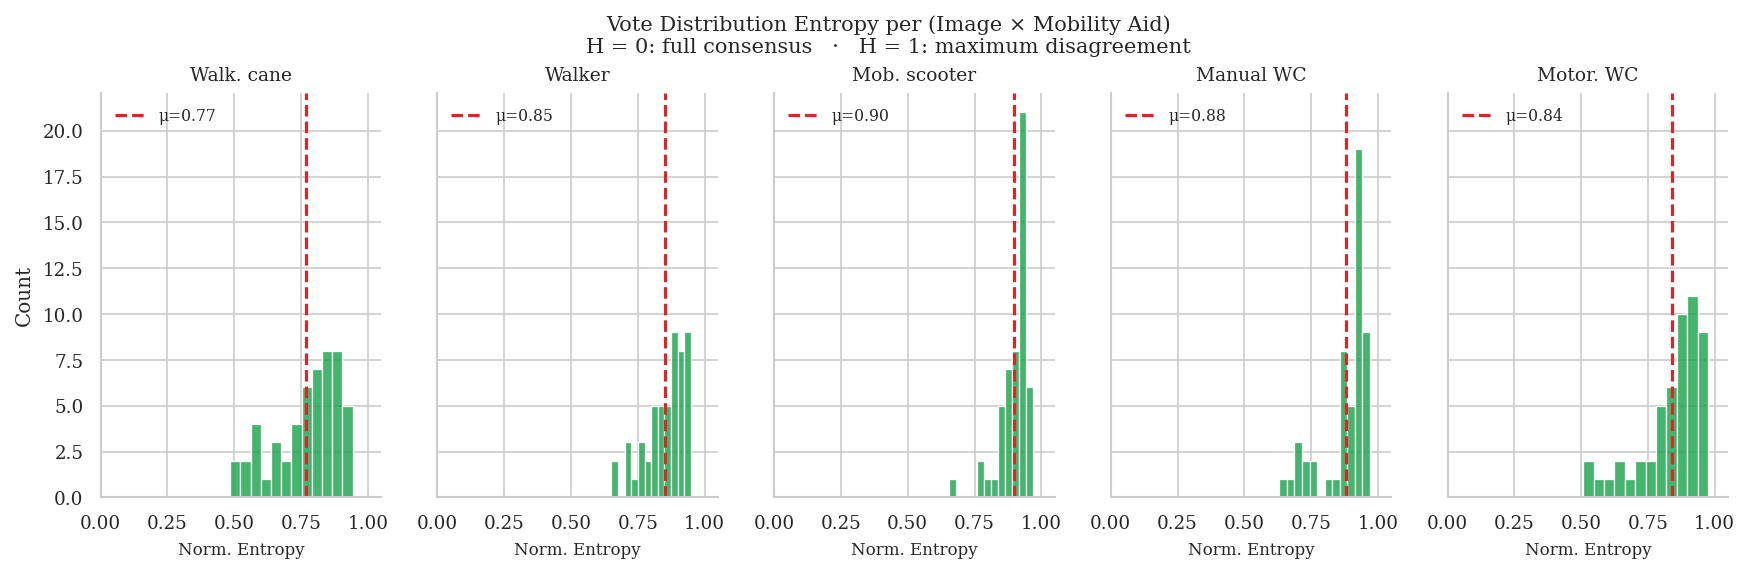
\includegraphics[width=\linewidth]{images/fig5_entropy_histogram.png}
\caption{Normalised vote entropy per (image, aid) pair for all five mobility aids. Dashed red line = per-aid mean. Consistently high entropy across all aids confirms that soft-label training is warranted and that hard majority labels discard genuine information.}
\label{fig:entropy}
\end{figure}

\begin{figure}[!t]
\centering
\begin{subfigure}[t]{0.48\linewidth}
\centering
\vspace{0pt}
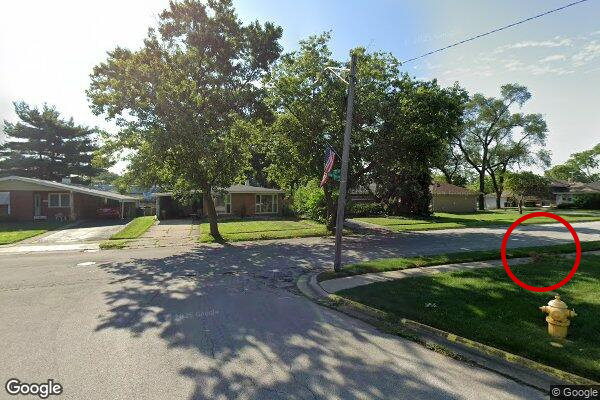
\includegraphics[width=\linewidth,height=2.6cm,keepaspectratio]{images/View1_Circle.jpg}
\caption{Sparse cue: missing curb ramp at intersection. Manual WC ``no'' = 78\%.}
\end{subfigure}
\hfill
\begin{subfigure}[t]{0.48\linewidth}
\centering
\vspace{0pt}
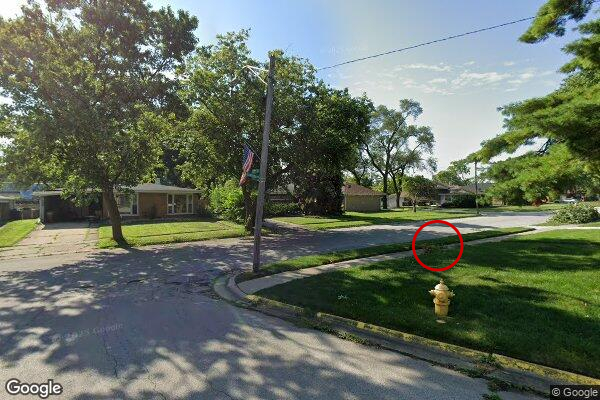
\includegraphics[width=\linewidth,height=2.6cm,keepaspectratio]{images/View2_Circle.jpg}
\caption{Similar scene, but the lawn-strip transition is passable. Manual WC ``yes'' = 61\%.}
\end{subfigure}
\\[0.3em]
\begin{subfigure}[t]{0.48\linewidth}
\centering
\vspace{0pt}
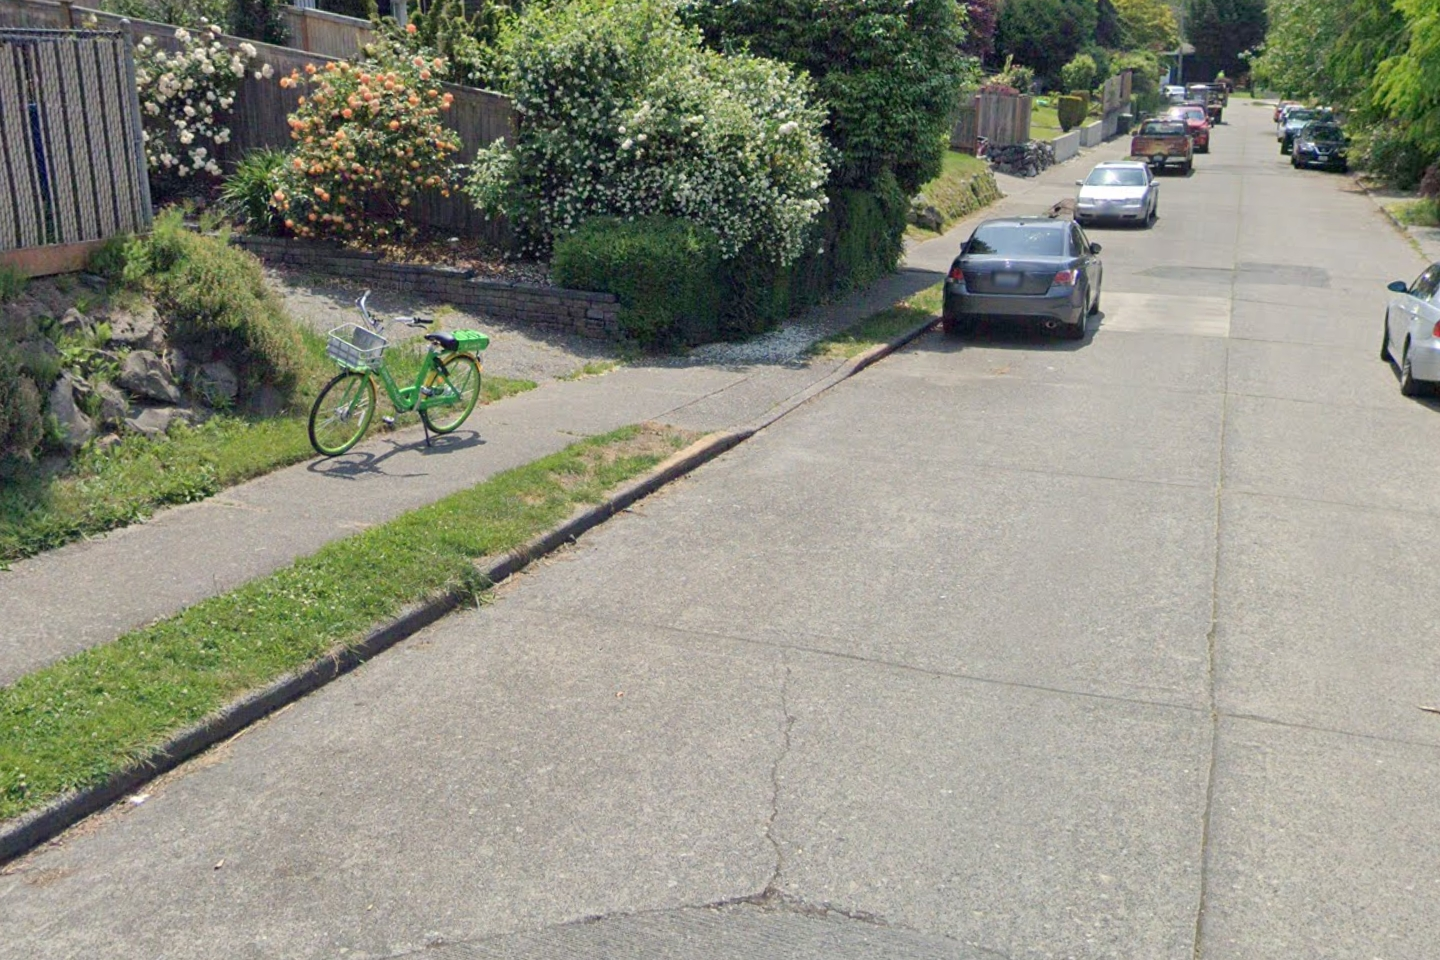
\includegraphics[width=\linewidth,height=2.6cm,keepaspectratio]{images/example2.jpg}
\caption{Clean continuous concrete; high inter-aid agreement on ``yes.''}
\end{subfigure}
\hfill
\begin{subfigure}[t]{0.48\linewidth}
\centering
\vspace{0pt}
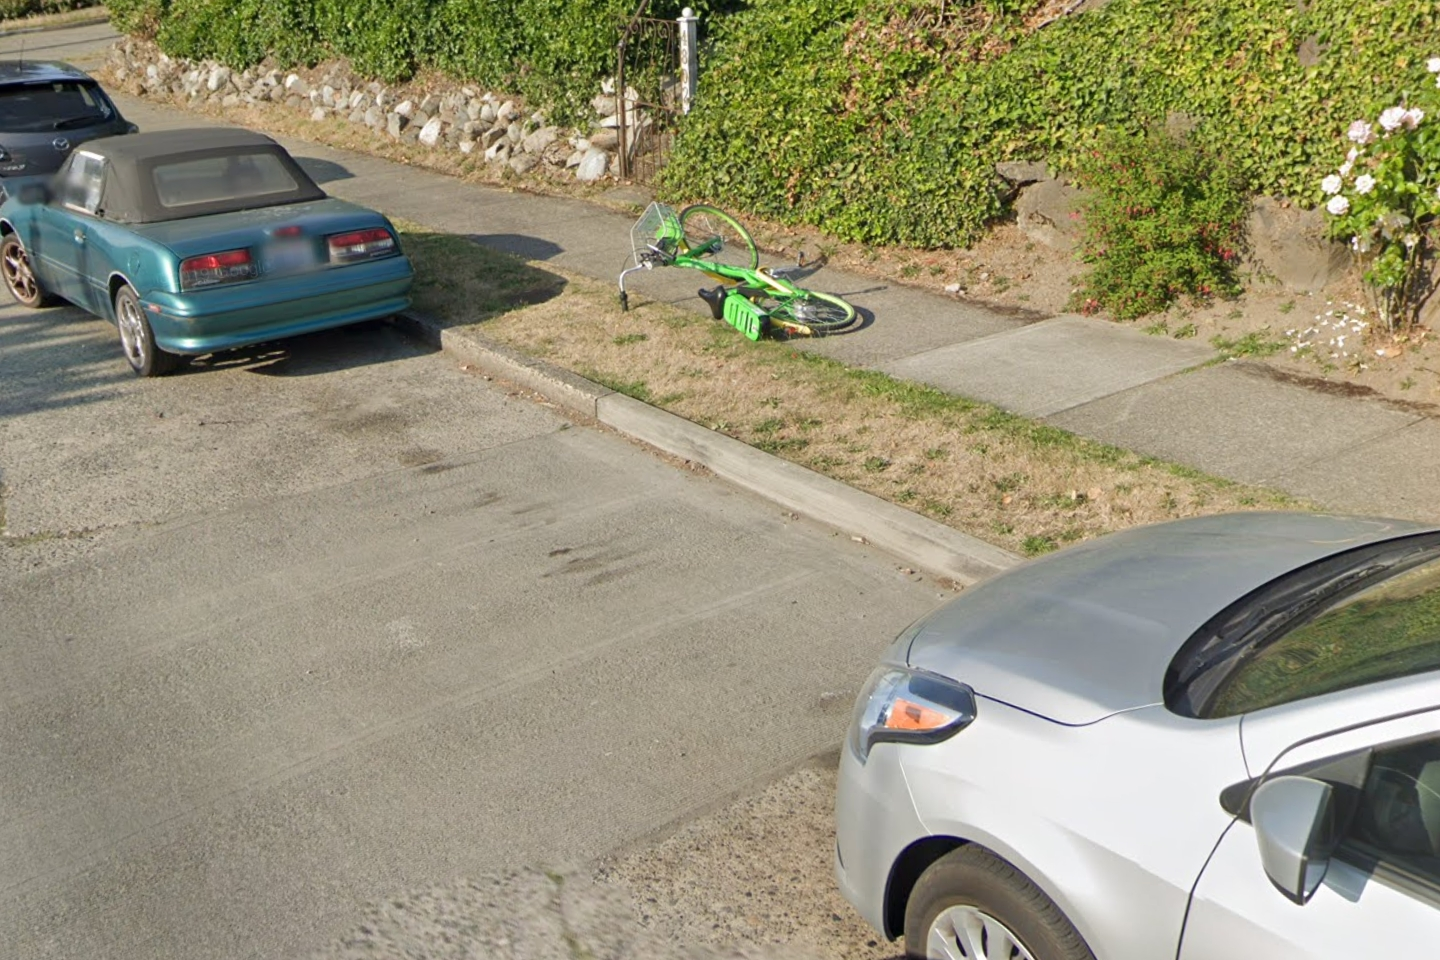
\includegraphics[width=\linewidth,height=2.6cm,keepaspectratio]{images/example3.jpg}
\caption{Driveway obstruction with vehicles and debris. Manual WC ``no'' = 56\%, cane ``yes'' = 64\%.}
\end{subfigure}
\caption{Representative Project Sidewalk audit views illustrating per-aid disagreement. Red circles mark the focal region the audit user is asked to assess. Adjacent panoramas with near-identical global appearance can produce sharply different per-aid vote distributions, motivating the joint per-aid soft-label formulation in Eq.~\ref{eq:softkl}.}
\label{fig:sidewalk_examples}
\end{figure}

\subsection{Image Pipeline}
\label{sec:data:pipeline}

\textbf{From panorama to view.} Each of the 52 audit views is produced by selecting one $90^\circ$ window of a Google Street View equirectangular panorama at the audit's known capture location, then deprojecting that window to a $640\times640$ rectilinear (undistorted) image. The window is centred on the audited sidewalk region using the human-drawn reference polygon supplied by Project Sidewalk. This single deprojected view is the only image the model sees for that scene, and is also the exact image shown to the audit users when they voted.

\textbf{Geometric verification.} A YOLOv12-seg model~\cite{tian2025yolov12attentioncentricrealtimeobject} trained on Project Sidewalk masks isolates the sidewalk and curb-ramp regions in each view. We retain only views where the predicted segmentation mask satisfies the area-ratio constraint $A_{\mathrm{pred}}/A_{\mathrm{gt}} \in [0.7, 1.3]$ against the reference polygon, filtering out severely viewpoint-distorted or mis-aligned deprojections. 52 of an initial $\sim$60 candidate views survive this geometric check and become the dataset used for both human voting and model training. All train/test splits are performed at the image (panorama) level with seed = 42, so a given scene appears in exactly one fold of the cross-validation.

\FloatBarrier
\section{Method}
\label{sec:method}

\subsection{Linear Probe on Frozen Encoders}

Each image $x_i$ is embedded by a frozen encoder $E$ and L2-normalised: $\mathbf{f}_i = E(x_i)/\|E(x_i)\|_2$. A per-aid linear head produces predictions:
\begin{equation}
\hat{\mathbf{y}}_{i,a} = \mathrm{softmax}(W_a\,\mathbf{f}_i + b_a).
\end{equation}
Encoder weights are never updated. We evaluate eight encoders: CLIP ViT-B/32, ViT-B/16, and ViT-L/14~\cite{radford2021learningtransferablevisualmodels}; DINOv2-base and DINOv2-large~\cite{oquab2023dinov2}; SigLIP2-base and SigLIP2-SO400M~\cite{tschannen2025siglip2}; and supervised ViT-B/16 from timm~\cite{dosovitskiy2021an}.

\subsection{Soft-KL Divergence Training}

The primary loss minimises the entropy-weighted KL divergence from model output to human vote distribution:
\begin{equation}
\mathcal{L}_{\mathrm{Soft\text{-}KL}} = \sum_{i,a} w_{i,a}\;\kl\!\bigl(\mathbf{y}_{i,a} \;\|\; \hat{\mathbf{y}}_{i,a}\bigr).
\label{eq:softkl}
\end{equation}
Unlike knowledge distillation, where soft targets come from a teacher model, the targets here are empirical human distributions backed by $\approx 190$ independent judgments each. The predicted $\hat{\mathbf{y}}_{i,a}$ is directly interpretable as ``the fraction of users in our study who would consider this sidewalk accessible.''

\subsection{Hard Cross-Entropy Baseline}

For comparison, we collapse each vote distribution to its argmax label $\hat{c}_{i,a} = \arg\max \mathbf{y}_{i,a}$ and train with standard cross-entropy:
\begin{equation}
\mathcal{L}_{\mathrm{Hard\text{-}CE}} = \sum_{i,a} w_{i,a}\;\mathrm{CE}\!\bigl(\hat{c}_{i,a},\,\hat{\mathbf{y}}_{i,a}\bigr).
\end{equation}
The entropy weight is retained so the comparison isolates the effect of the target (distribution vs.\ hard label) rather than the weighting.

\subsection{Calibration Metric: Soft Brier Score}

We assess calibration against the human vote distribution:
\begin{equation}
\brier = \frac{1}{N}\sum_{i,a} \bigl\|\hat{\mathbf{y}}_{i,a} - \mathbf{y}_{i,a}\bigr\|_2^2.
\label{eq:brier}
\end{equation}
Lower is better. A model with $\brier = 0.07$ that outputs $\hat{p}_\mathrm{yes} = 0.65$ for a sidewalk where 62\% of users voted ``yes'' is providing actionable probabilistic information. A model with $\brier = 0.23$ outputting $\hat{p}_\mathrm{yes} = 0.97$ for the same image misleads any downstream planner that treats the score as a probability.

\subsection{Training Details}
\label{sec:method:training}

All probes use AdamW (lr $= 10^{-3}$, weight decay $= 10^{-4}$, 50 epochs, batch size 64). Encoder weights are frozen. \textbf{5-fold cross-validation} at the panorama level prevents leakage between rectified crops from the same location. Global seed = 42. All experiments run on a single NVIDIA A100 40 GB GPU. Figure~\ref{fig:pipeline} summarises the full pipeline.

\begin{figure*}[!t]
\centering
\resizebox{\textwidth}{!}{%
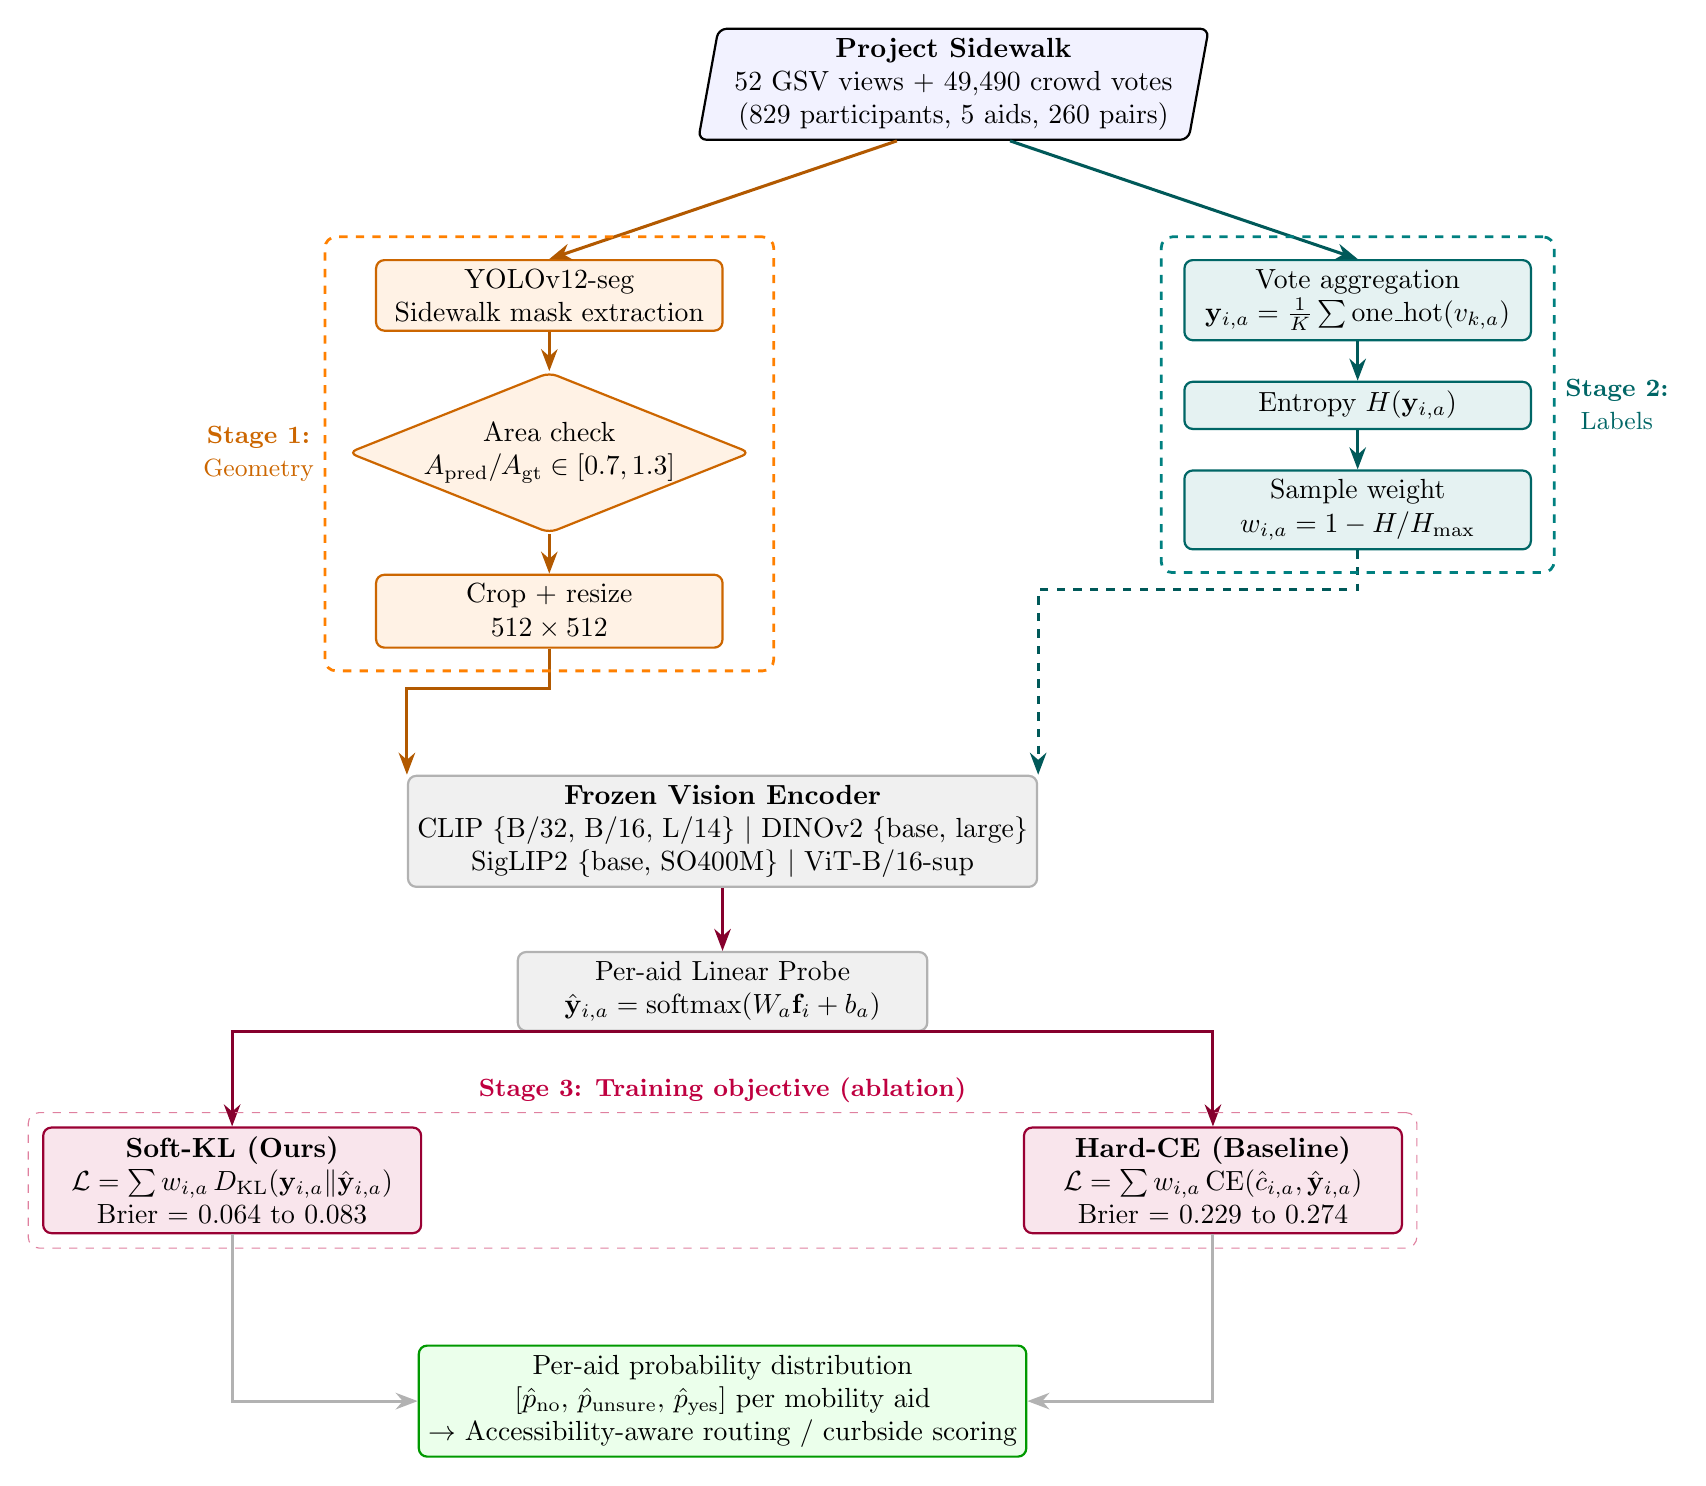
\begin{tikzpicture}[node distance=5mm, font=\normalsize, >=Stealth]
\tikzset{
  base/.style={draw, align=center, line width=0.8pt, rounded corners=3pt},
  io/.style={base, fill=blue!5, trapezium, trapezium left angle=80, trapezium right angle=100, trapezium stretches=true, minimum height=1cm, minimum width=6.5cm},
  geometry/.style={base, fill=orange!10, draw=orange!80!black, minimum width=4.4cm},
  labels/.style={base, fill=teal!10, draw=teal!80!black, minimum width=4.4cm},
  encoder/.style={base, fill=gray!12, draw=gray!60, minimum width=5.2cm},
  method/.style={base, fill=purple!10, draw=purple!80!black, minimum width=4.8cm},
  output/.style={base, fill=green!8, draw=green!60!black, minimum width=5.5cm},
  arrow/.style={->, thick, draw=gray!60, line width=1.1pt},
  arrow_geo/.style={->, thick, draw=orange!70!black, line width=1.1pt},
  arrow_lab/.style={->, thick, draw=teal!70!black, line width=1.1pt},
  arrow_mod/.style={->, thick, draw=purple!70!black, line width=1.1pt},
}

% Input
\node (data) [io] {\textbf{Project Sidewalk}\\52 GSV views + 49{,}490 crowd votes\\(829 participants, 5 aids, 260 pairs)};

% Stage 1: Geometry
\node (seg) [geometry, below left=15mm and 22mm of data] {YOLOv12-seg\\Sidewalk mask extraction};
\node (verify) [geometry, below=of seg, diamond, aspect=2.5, inner sep=0pt] {Area check\\$A_{\text{pred}}/A_{\text{gt}} \in [0.7,1.3]$};
\node (crop) [geometry, below=of verify] {Crop + resize\\$512 \times 512$};

% Stage 2: Labels
\node (agg) [labels, below right=15mm and 22mm of data] {Vote aggregation\\$\mathbf{y}_{i,a}=\frac{1}{K}\sum \mathrm{one\_hot}(v_{k,a})$};
\node (ent) [labels, below=of agg] {Entropy $H(\mathbf{y}_{i,a})$};
\node (wgt) [labels, below=of ent] {Sample weight\\$w_{i,a}=1-H/H_{\max}$};

% Stage 1 arrows
\draw[arrow_geo] (data.south west) -- (seg.north);
\draw[arrow_geo] (seg) -- (verify);
\draw[arrow_geo] (verify) -- (crop);
\draw[arrow_lab] (data.south east) -- (agg.north);
\draw[arrow_lab] (agg) -- (ent);
\draw[arrow_lab] (ent) -- (wgt);

% Frozen Encoder
\node (enc) [encoder, below=16mm of crop, xshift=22mm] {\textbf{Frozen Vision Encoder}\\CLIP \{B/32, B/16, L/14\} $|$ DINOv2 \{base, large\}\\SigLIP2 \{base, SO400M\} $|$ ViT-B/16-sup};
\draw[arrow_geo] (crop.south) -- ++(0,-5mm) -| (enc.north west);
\draw[arrow_lab, dashed] (wgt.south) -- ++(0,-5mm) -| (enc.north east);

% Linear Probe
\node (probe) [encoder, below=8mm of enc] {Per-aid Linear Probe\\$\hat{\mathbf{y}}_{i,a}=\mathrm{softmax}(W_a\mathbf{f}_i+b_a)$};
\draw[arrow_mod] (enc) -- (probe);

% Two training branches
\node (softkl) [method, below left=12mm and 12mm of probe] {\textbf{Soft-KL (Ours)}\\$\mathcal{L}=\sum w_{i,a}\,D_{\mathrm{KL}}(\mathbf{y}_{i,a}\|\hat{\mathbf{y}}_{i,a})$\\Brier = 0.064 to 0.083};
\node (hardce) [method, below right=12mm and 12mm of probe] {\textbf{Hard-CE (Baseline)}\\$\mathcal{L}=\sum w_{i,a}\,\mathrm{CE}(\hat{c}_{i,a},\hat{\mathbf{y}}_{i,a})$\\Brier = 0.229 to 0.274};
\draw[arrow_mod] (probe.south) -| (softkl.north);
\draw[arrow_mod] (probe.south) -| (hardce.north);

% Output
\coordinate (outmid) at ($(softkl.south)!0.5!(hardce.south)$);
\node (out) [output, below=14mm of outmid] {Per-aid probability distribution\\$[\hat{p}_\mathrm{no},\,\hat{p}_\mathrm{unsure},\,\hat{p}_\mathrm{yes}]$ per mobility aid\\$\rightarrow$ Accessibility-aware routing / curbside scoring};
\draw[arrow] (softkl.south) |- (out.west);
\draw[arrow] (hardce.south) |- (out.east);

% Dashed boxes
\node[draw=orange, dashed, line width=1pt, rounded corners, fit=(seg)(verify)(crop), inner sep=8pt, label={[orange!80!black, align=center]west:\small\textbf{Stage 1:}\\\small Geometry}] {};
\node[draw=teal, dashed, line width=1pt, rounded corners, fit=(agg)(ent)(wgt), inner sep=8pt, label={[teal!80!black, align=center]east:\small\textbf{Stage 2:}\\\small Labels}] {};
\node[draw=purple!50, dashed, rounded corners, fit=(softkl)(hardce), inner sep=5pt, label={[purple, font=\small]north:\textbf{Stage 3: Training objective (ablation)}}] {};

\end{tikzpicture}%
}
\caption{End-to-end pipeline. Panoramas are deprojected, segmented, and verified on the left (orange); crowdsourced votes are aggregated into probability distributions with entropy-derived sample weights on the right (teal). Both feed a shared frozen vision encoder (one of 8 evaluated) followed by a per-aid linear probe. Training objective is either Soft-KL (ours, Brier 0.064 to 0.083) or Hard-CE (baseline, Brier 0.229 to 0.274). The output is a calibrated per-aid distribution over \{no, unsure, yes\} that feeds downstream accessibility-aware routing.}
\label{fig:pipeline}
\end{figure*}

\section{Results}
\label{sec:results}

We report results in the order that matters for the planner: calibration first, classification accuracy second. All numbers below are 5-fold panorama-level CV at seed = 42; the $\pm$ values are 95\% confidence intervals computed from the per-fold per-aid distribution ($n=40$ fold-aid measurements per encoder), not nominal standard errors. The training images are few (52), but the claim is not visual foundation-model learning: it is whether frozen urban-scene features can be calibrated to dense human vote distributions, and whether those calibrated probabilities improve a pedestrian planner.

\subsection{Calibration: Soft-KL vs.\ Hard-CE (Headline)}
\label{sec:calibration_headline}

Table~\ref{tab:calibration_headline} reports the primary calibration result: across all eight encoders and both training objectives, Soft-KL achieves a soft Brier score $3\times$ lower than Hard-CE on the same encoder and the same folds. The Brier gap is large relative to its confidence interval; the gap is not driven by any single encoder.

\begin{table}[!t]
\caption{\textbf{Headline calibration result.} Soft Brier ($\downarrow$, lower = better calibrated against the human vote distribution). 5-fold CV; $\pm$ is 95\% CI over the 40 (fold, aid) measurements per encoder. \textbf{Bold}: best within its column. The Soft-KL/Hard-CE gap is consistent across all eight encoders.}
\label{tab:calibration_headline}
\centering\small
\setlength{\tabcolsep}{4pt}
\resizebox{\columnwidth}{!}{%
\begin{tabular}{@{}lccc@{}}
\toprule
\textbf{Encoder} & \textbf{Brier (Soft-KL)} & \textbf{Brier (Hard-CE)} & \textbf{Ratio} \\
\midrule
CLIP B/32      & $\mathbf{0.064\pm0.011}$ & $0.231\pm0.016$ & $3.6\times$ \\
DINOv2-large   & $0.075\pm0.013$         & $0.253\pm0.023$ & $3.4\times$ \\
SigLIP2-SO400M & $0.066\pm0.014$         & $0.256\pm0.022$ & $3.9\times$ \\
DINOv2-base    & $0.080\pm0.010$         & $0.238\pm0.024$ & $3.0\times$ \\
SigLIP2-base   & $0.082\pm0.011$         & $\mathbf{0.228\pm0.020}$ & $2.8\times$ \\
CLIP L/14      & $0.080\pm0.011$         & $0.230\pm0.022$ & $2.9\times$ \\
ViT-B/16-sup   & $0.083\pm0.015$         & $0.274\pm0.027$ & $3.3\times$ \\
CLIP B/16      & $0.080\pm0.017$         & $0.239\pm0.025$ & $3.0\times$ \\
\midrule
\textit{Mean}  & $0.076$                 & $0.244$         & $\mathbf{3.2\times}$ \\
\bottomrule
\end{tabular}%
}
\end{table}

For a routing planner this gap is concrete: an edge with $\hat{p}_\mathrm{yes}=0.55$ incurs $4\times$ the accessibility penalty of one with $\hat{p}_\mathrm{yes}=0.91$ at our chosen $\beta_c=8$ (\S\ref{sec:routing}). Hard-CE probes overwhelmingly output $\hat{p}_\mathrm{yes}\in\{$near $0.0$, near $1.0\}$ regardless of the underlying vote distribution, the same overconfidence pattern documented by Guo et al.~\cite{guo2017calibration} for modern networks, which collapses the routing gradient. Soft-KL preserves the empirical bimodality and gives the planner a usable continuous risk signal. We emphasise that this is the metric the downstream planner directly consumes.

\subsection{Encoder Comparison (F1, secondary)}
\label{sec:encoder}

For completeness, and for comparability with prior work that trains on hard labels, Table~\ref{tab:main} reports macro-F1 under Hard-CE training. We note up-front: F1 is a secondary descriptor here because the planner does not consume argmax labels, and Soft-KL's redistribution onto ``unsure'' is penalised under F1 by construction (no image in the dataset has ``unsure'' as the majority vote, so any probability mass placed there cannot win the argmax).

\begin{table}[!t]
\caption{\textbf{Hard-CE macro-F1 per encoder.} 5-fold CV, seed = 42. WC = wheelchair. ``Overall'' is the mean across five aids; $\pm$ is 95\% CI over the 40 (fold, aid) measurements. Most encoders are statistically indistinguishable from each other on overall F1; the encoder rank-ordering is therefore not a strong claim of this paper.}
\label{tab:main}
\centering\small
\setlength{\tabcolsep}{3.5pt}
\resizebox{\columnwidth}{!}{%
\begin{tabular}{@{}lccccc|c@{}}
\toprule
\textbf{Encoder} & \textbf{Cane} & \textbf{Walk.} & \textbf{Scoot.} & \textbf{Man.WC} & \textbf{Mot.WC} & \textbf{Overall} \\
\midrule
CLIP B/32      & 0.453 & \textbf{0.761} & 0.558 & \textbf{0.675} & 0.639 & $\mathbf{0.617\pm0.059}$ \\
DINOv2-base    & 0.446 & 0.720 & 0.668 & 0.574 & \textbf{0.664} & $0.614\pm0.069$ \\
DINOv2-large   & 0.489 & 0.675 & \textbf{0.746} & 0.502 & 0.652 & $0.613\pm0.059$ \\
SigLIP2-base   & 0.458 & 0.700 & 0.587 & 0.572 & 0.664 & $0.596\pm0.060$ \\
CLIP L/14      & 0.453 & 0.707 & 0.698 & 0.523 & 0.597 & $0.595\pm0.064$ \\
ViT-B/16-sup   & \textbf{0.513} & 0.682 & 0.606 & 0.553 & 0.509 & $0.573\pm0.070$ \\
SigLIP2-SO400M & 0.453 & 0.669 & 0.519 & 0.483 & 0.652 & $0.555\pm0.064$ \\
CLIP B/16      & 0.434 & 0.536 & 0.569 & 0.562 & 0.618 & $0.544\pm0.068$ \\
\bottomrule
\end{tabular}%
}
\end{table}

CLIP ViT-B/32, DINOv2-base, and DINOv2-large all land within their 95\% CIs of each other on overall F1, so we do not claim a strict encoder ranking. What is robust is the pattern: dense self-supervised features (DINOv2-large achieves the highest single-cell score, Mobility Scooter $= 0.746$) and contrastive language-image features (CLIP B/32 leads Walker $= 0.761$) both score above the ImageNet-supervised features (ViT-B/16-sup, overall $0.573$), with the latter ranking sixth despite sharing its architecture with CLIP B/16. The plausible reading is that traversability perception requires either spatial-density or semantic-priors pretraining; ImageNet class-discriminative pretraining transfers less effectively to this task. Figure~\ref{fig:heatmap} visualises the full matrix under Soft-KL, where the encoder ranking inverts (DINOv2-large leads; see \S\ref{sec:ablation} for the interpretation of this inversion as a calibration vs.\ argmax distinction).

\begin{figure}[!t]
\centering
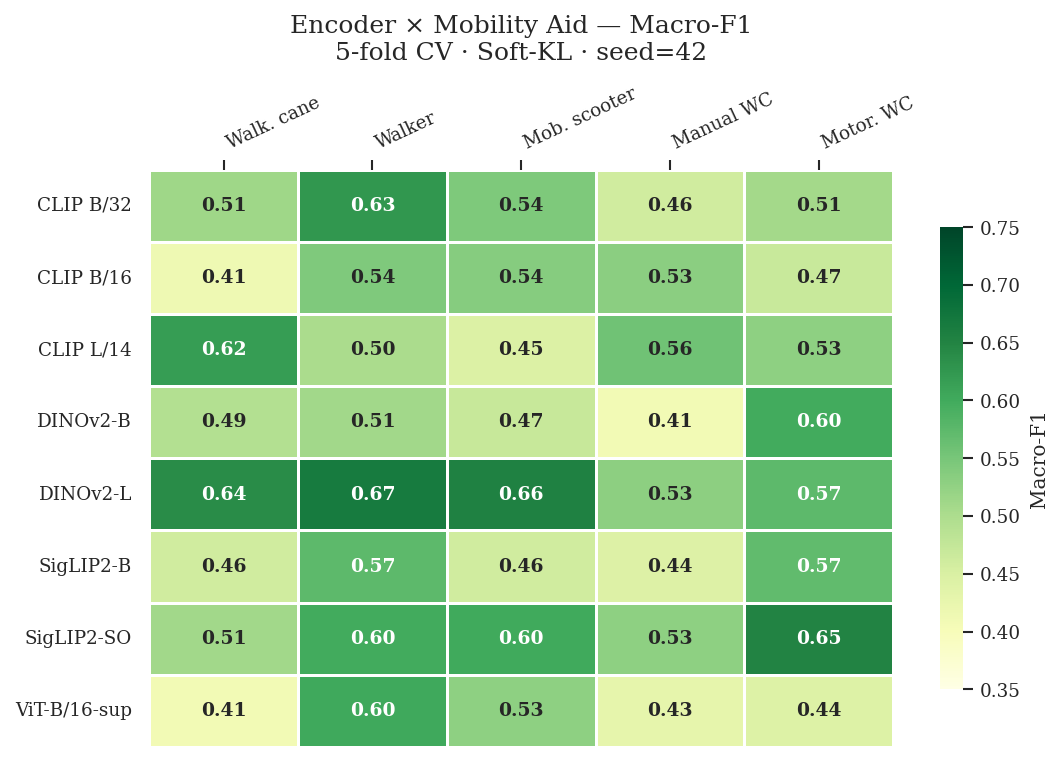
\includegraphics[width=\linewidth]{images/fig1_encoder_f1_heatmap.png}
\caption{Encoder $\times$ mobility aid macro-F1 heatmap under Soft-KL. DINOv2-large shows the most consistent per-aid coverage. Walking cane is the hardest aid for every encoder, reflecting its 6.4:1 yes-to-no imbalance.}
\label{fig:heatmap}
\end{figure}

\subsection{Soft-KL vs.\ Hard-CE Ablation}
\label{sec:ablation}

Table~\ref{tab:ablation} isolates the effect of the training objective across all eight encoders.

\begin{table}[!t]
\caption{\textbf{Ablation: Soft-KL vs.\ Hard-CE.} $\Delta$F1 = Hard-CE F1 $-$ Soft-KL F1 (positive = Hard-CE wins argmax); $\pm$ is 95\% CI over 40 (fold, aid) measurements. Brier values shown are Soft-KL; Hard-CE Brier is reported in Table~\ref{tab:calibration_headline}. Notably the F1 gap is within or near the CI for every encoder, while the Brier gap is large for all.}
\label{tab:ablation}
\centering\small
\setlength{\tabcolsep}{4pt}
\resizebox{\columnwidth}{!}{%
\begin{tabular}{@{}lccc|c@{}}
\toprule
\textbf{Encoder} & \textbf{Soft-KL F1} & \textbf{Hard-CE F1} & \textbf{$\Delta$F1} & \textbf{Brier $\downarrow$} \\
\midrule
CLIP B/32      & $0.530\pm0.067$ & $\mathbf{0.617\pm0.059}$ & $+0.087$ & 0.064 \\
DINOv2-large   & $\mathbf{0.613\pm0.071}$ & $0.613\pm0.059$ & $0.000$ & 0.075 \\
SigLIP2-SO400M & $\mathbf{0.579\pm0.064}$ & $0.555\pm0.064$ & $-0.024$ & 0.066 \\
DINOv2-base    & $0.496\pm0.064$ & $\mathbf{0.614\pm0.069}$ & $+0.118$ & 0.080 \\
SigLIP2-base   & $0.502\pm0.057$ & $\mathbf{0.596\pm0.060}$ & $+0.094$ & 0.082 \\
CLIP L/14      & $0.531\pm0.065$ & $\mathbf{0.595\pm0.064}$ & $+0.064$ & 0.080 \\
ViT-B/16-sup   & $0.482\pm0.073$ & $\mathbf{0.573\pm0.070}$ & $+0.091$ & 0.083 \\
CLIP B/16      & $0.499\pm0.060$ & $\mathbf{0.544\pm0.068}$ & $+0.045$ & 0.080 \\
\midrule
\textit{Mean}  & $0.529$         & $\mathbf{0.588}$        & $+0.059$ & $\mathbf{0.076}$ \\
\bottomrule
\end{tabular}%
}
\end{table}

Hard-CE yields higher argmax F1 in six of eight cases ($+$0.059 on average). The explanation is structural: no image in the dataset has ``unsure'' as the majority vote; the class never exceeds 50\% for any (image, aid) pair. Soft-KL distributes probability mass onto ``unsure'' to faithfully mirror the human distribution, but macro-F1 is computed from argmax predictions and never rewards this redistribution. Because the majority label is always either ``yes'' or ``no'' by construction, Soft-KL's spread over three classes always looks like hedging under F1, regardless of whether that spread is epistemically correct. This is a property of the metric and the label structure, not evidence that Soft-KL is learning incorrectly.

The calibration story reverses entirely: Soft-KL achieves Brier = 0.064 to 0.083 versus 0.229 to 0.274 for Hard-CE, a 3$\times$ difference sustained across all eight encoders (Figure~\ref{fig:brier}). For a routing planner, the distinction is concrete: a model outputting $\hat{p}_\mathrm{yes} = 0.65$ for a sidewalk where 62\% of users voted ``yes'' provides useful risk information. A model confidently outputting $\hat{p}_\mathrm{yes} = 0.97$ for the same image is providing false certainty that misrepresents genuine human disagreement. The encoder ranking also inverts between objectives: DINOv2-large leads Soft-KL (0.613) but ties third under Hard-CE (0.613), while CLIP-B/32 leads Hard-CE but falls fourth under Soft-KL (0.530). This inversion indicates that DINOv2 features better capture the uncertainty structure of human accessibility judgments, while CLIP features better predict the majority class.

\begin{figure}[!t]
\centering
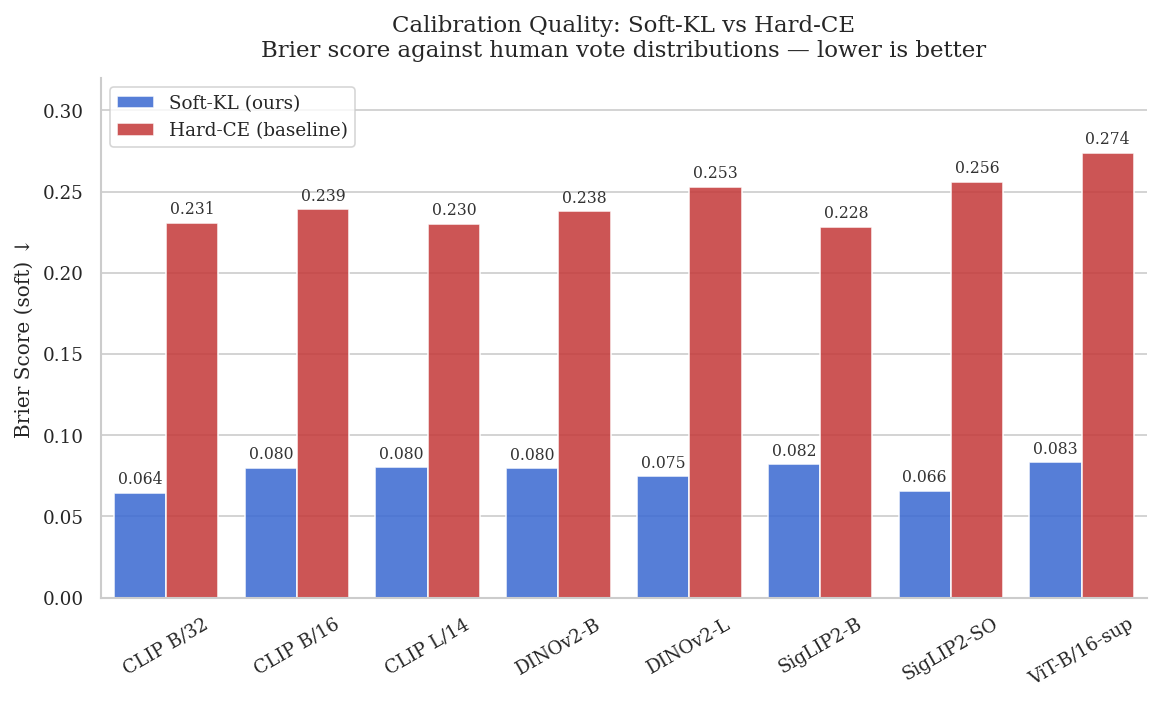
\includegraphics[width=\linewidth]{images/fig2_brier_comparison.png}
\caption{Soft Brier score per encoder: Soft-KL (blue) vs.\ Hard-CE (red). Lower is better calibration. The 3$\times$ gap is consistent across all eight encoders; Hard-CE produces overconfident predictions that misrepresent genuine human uncertainty.}
\label{fig:brier}
\end{figure}

\subsection{Zero-Shot VLM Comparison}
\label{sec:zeroshot}

Three VLMs are evaluated without any task-specific training data (Table~\ref{tab:zeroshot}). A structured natural-language prompt is used for each aid; free-text model responses are parsed to ternary labels via keyword matching (prompt variants detailed in the Supplementary).

\begin{table}[!t]
\caption{Trained probes vs.\ zero-shot VLMs. F1 = mean across 5 aids. Brier = soft Brier against human vote distributions. Probe latency = feature extraction only (single image, A100).}
\label{tab:zeroshot}
\centering\small
\setlength{\tabcolsep}{4pt}
\resizebox{\columnwidth}{!}{%
\begin{tabular}{@{}lcccc@{}}
\toprule
\textbf{Method} & \textbf{F1} & \textbf{Bal.Acc} & \textbf{Brier $\downarrow$} & \textbf{Latency (ms)} \\
\midrule
\multicolumn{5}{l}{\textit{Trained linear probes (5-fold CV)}} \\
CLIP B/32 + Hard-CE         & \textbf{0.617} & n/a   & 0.231 &  61.6 \\
DINOv2-large + Soft-KL      & 0.613          & n/a   & \textbf{0.075} &  78.5 \\
\midrule
\multicolumn{5}{l}{\textit{Zero-shot VLMs (no training data)}} \\
Qwen3-VL-8B   & 0.576 & 0.633 & 0.468 & 6{,}182 \\
LLaVA-1.5-7B  & 0.418 & 0.508 & 0.423 &   135  \\
Qwen2.5-VL-7B & 0.412 & 0.596 & 0.632 &   185  \\
\bottomrule
\end{tabular}%
}
\end{table}

The best zero-shot VLM (Qwen3-VL-8B) reaches F1 = 0.576, only 0.041 below the best trained probe. However, its Brier score is 0.468, or 6.2$\times$ worse calibration than DINOv2-large Soft-KL (0.075), and at 6.2\,s per image it cannot meet the latency budget for real-time edge scoring. LLaVA-1.5-7B and Qwen2.5-VL-7B have balanced accuracy near 0.5, consistent with majority-class bias. Prompt sensitivity is non-trivial (6--11\% relative F1 variation per model; full results in the Supplementary), further motivating task-specific trained probes over zero-shot queries for production routing. Figures~\ref{fig:zeroshot} and~\ref{fig:latency} show the comparison.

\begin{figure}[!t]
\centering
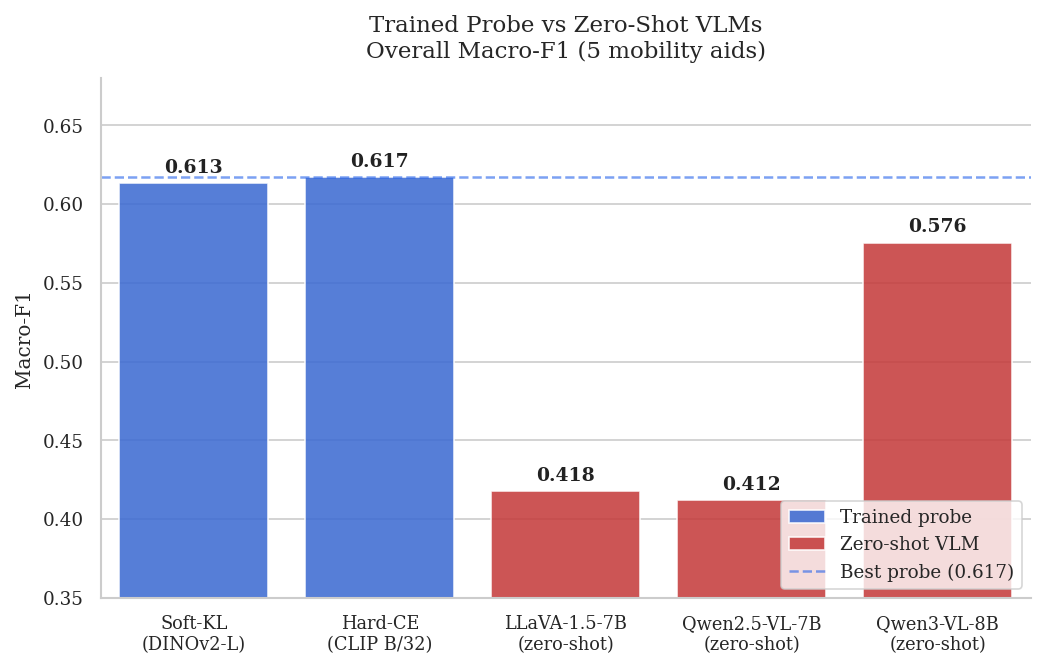
\includegraphics[width=\linewidth]{images/fig4_zeroshot_vs_probe.png}
\caption{Trained probes vs.\ zero-shot VLMs on overall macro-F1. Dashed blue line = best probe (0.617). Qwen3-VL-8B (0.576) comes within 0.041 F1 at the cost of 102$\times$ higher latency and 6.2$\times$ worse Brier score.}
\label{fig:zeroshot}
\end{figure}

\begin{figure}[!t]
\centering
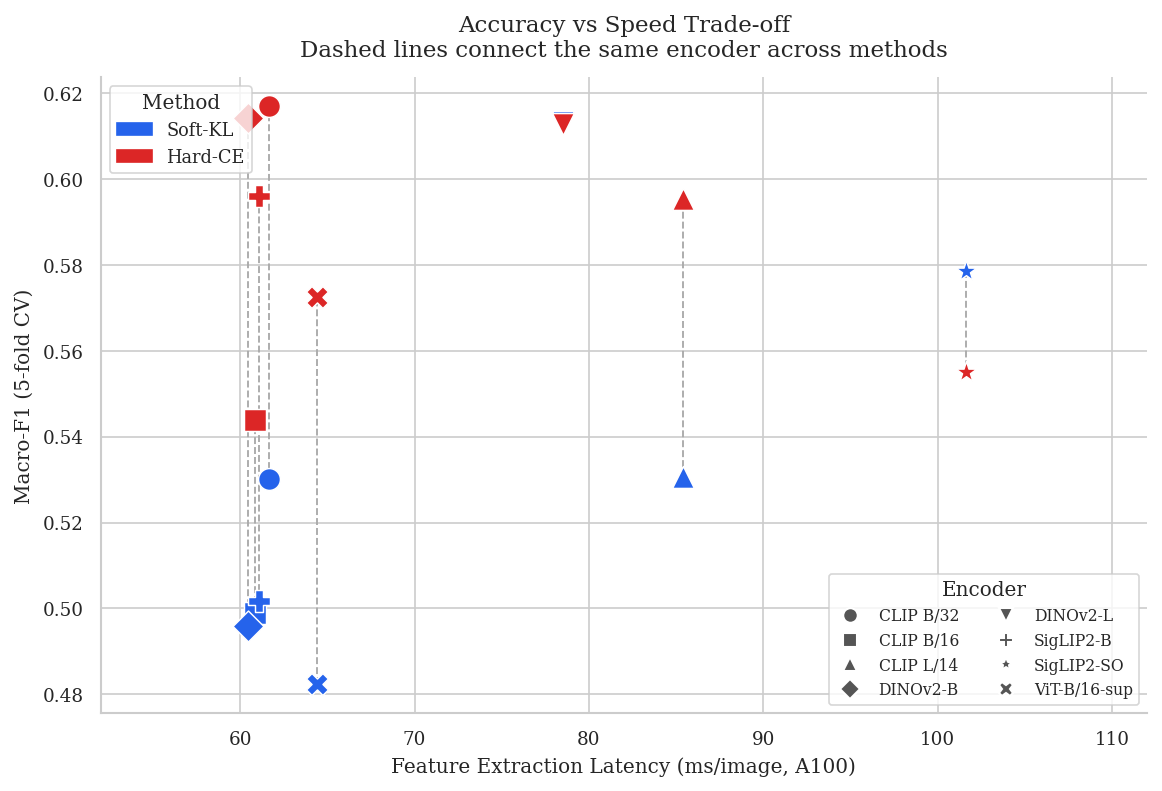
\includegraphics[width=\linewidth]{images/fig3_latency_vs_f1.png}
\caption{Macro-F1 vs.\ inference latency for all 8 encoders under Soft-KL (blue) and Hard-CE (red). DINOv2-large is Pareto-optimal under Soft-KL (78.5\,ms, F1 = 0.613). All encoder probes are within the real-time budget for routing applications.}
\label{fig:latency}
\end{figure}

\subsection{Generalization to Unseen Cities}
\label{sec:generalization}

As an auxiliary encoder-transfer check, distinct from the main per-aid traversability task, we evaluate whether DINOv2-large Soft-KL features generalize to a coarser binary label (CurbRamp / NoCurbRamp) from Project Sidewalk audits across four cities: Pittsburgh PA, Detroit MI, Zurich, and Taipei. This is not a test of the five-aid calibration objective; it is a geographic stress-test of the learned features on a related but simpler binary classification. No city-specific adaptation is applied; encoder and probe weights are identical to the Pittsburgh-trained model.

Table~\ref{tab:generalization} reports per-city balanced accuracy. All four cities exceed the 0.50 chance level. Within the US, Pittsburgh (0.566) and Detroit (0.570) produce nearly identical results, confirming transfer robustness rather than Pittsburgh-specific overfitting. Zurich achieves 0.616 (+11.6pp above chance), likely because the probe was trained on data including Amsterdam, a city with similar pedestrian infrastructure conventions. Taipei reaches only 0.518 (+1.8pp above chance), a result we report transparently as a boundary condition. The model's Western-centric training (US and European cities) does not transfer to substantially different East Asian urban morphologies, motivating future geographically diverse data collection. Figure~\ref{fig:generalization} visualises the per-city results.

\begin{table}[!t]
\caption{Generalization: DINOv2-large Soft-KL (trained on the 52-view passability benchmark) evaluated on binary CurbRamp labels across four unseen cities. Balanced accuracy; chance = 0.50.}
\label{tab:generalization}
\centering\small
\begin{tabular}{@{}llcc@{}}
\toprule
\textbf{City} & \textbf{Region} & \textbf{Bal.Acc} & \textbf{n} \\
\midrule
Pittsburgh & North America & 0.566 & 162 \\
Detroit    & North America & 0.570 & 91  \\
Zurich     & Europe        & 0.616 & 89  \\
Taipei     & Asia          & 0.518 & 95  \\
\midrule
\textbf{Overall} & n/a & \textbf{0.573} & \textbf{437} \\
\bottomrule
\end{tabular}
\end{table}

\begin{figure}[!t]
\centering
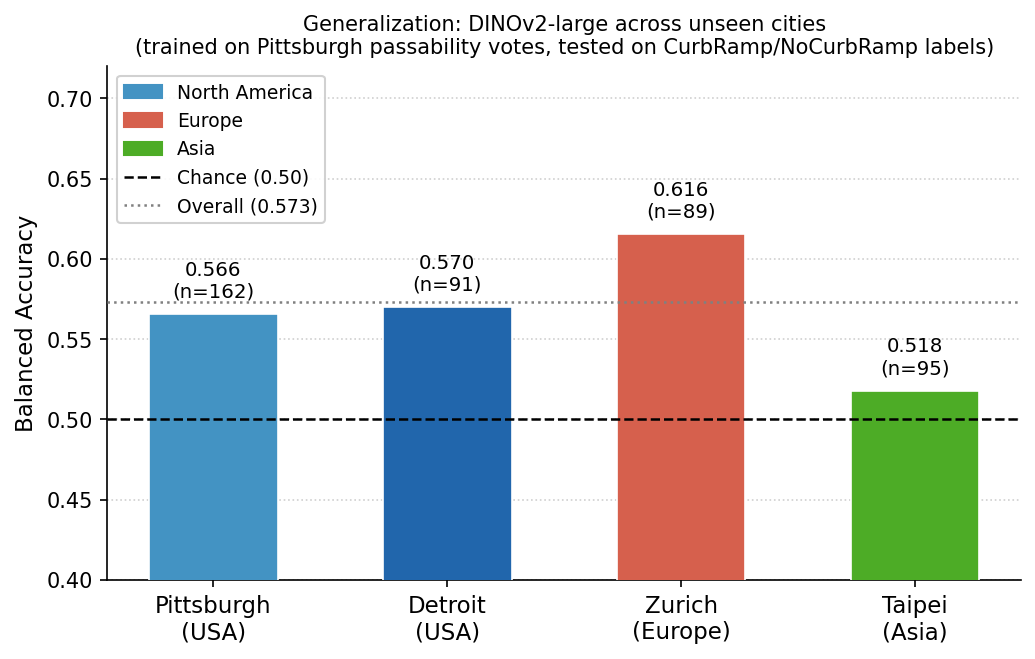
\includegraphics[width=\linewidth]{images/generalization_figure.png}
\caption{Generalization: balanced accuracy per city for DINOv2-large Soft-KL evaluated on binary CurbRamp labels in unseen cities. Dashed line = chance (0.50). Pittsburgh and Detroit are consistent (+6.6/+7.0pp), Zurich is stronger (+11.6pp), and Taipei reveals a Western-centric limitation (+1.8pp).}
\label{fig:generalization}
\end{figure}

\subsection{Walking Cane: Hard-CE Failure Under Class Imbalance}
\label{sec:cane}

Walking cane is the structural anomaly in Table~\ref{tab:main}: every encoder scores at or below the trivial majority-class baseline of 0.467 under Hard-CE, with the best result (ViT-B/16-sup, 0.513) only marginally above it. The cause is a 6.4:1 positive skew: 45 of 52 images have a majority-yes vote for walking cane. Hard-CE with entropy sample weights still learns to predict ``yes'' for nearly all inputs; the minority ``no'' class is effectively abandoned. This pattern holds for 6 of 8 encoders tested, confirming it is a systematic failure of the objective rather than an encoder-specific artifact. The two exceptions (CLIP-B/16 and ViT-B/16-sup) are the lowest-performing encoders overall; among encoders with overall F1 $\geq$ 0.530, Soft-KL gives higher walking-cane F1 than Hard-CE.

Soft-KL achieves F1 = 0.640 for walking cane (+0.187, +42\% relative), despite using the same features and training set. The mechanism is visible in Fig.~\ref{fig:cane_votes}: examining the 7 majority-``no'' images, 5 of 7 have human vote margins $<0.03$ between the top-two vote fractions, meaning annotators are nearly split 50/50. Hard-CE forces these borderline examples into hard negatives, creating contradictory training signals that collapse the model to the majority class. Soft-KL instead assigns these images soft targets $\approx [0.45, 0.05, 0.45]$, preserving the training signal from the 2 unambiguous ``no'' examples (margins 0.111 and 0.327) without being corrupted by the 5 ambiguous ones. The operationally critical implication: Hard-CE treats near-impassable edges as confidently safe for cane users; Soft-KL correctly signals them as uncertain and routes around them.

\begin{figure}[!t]
\centering
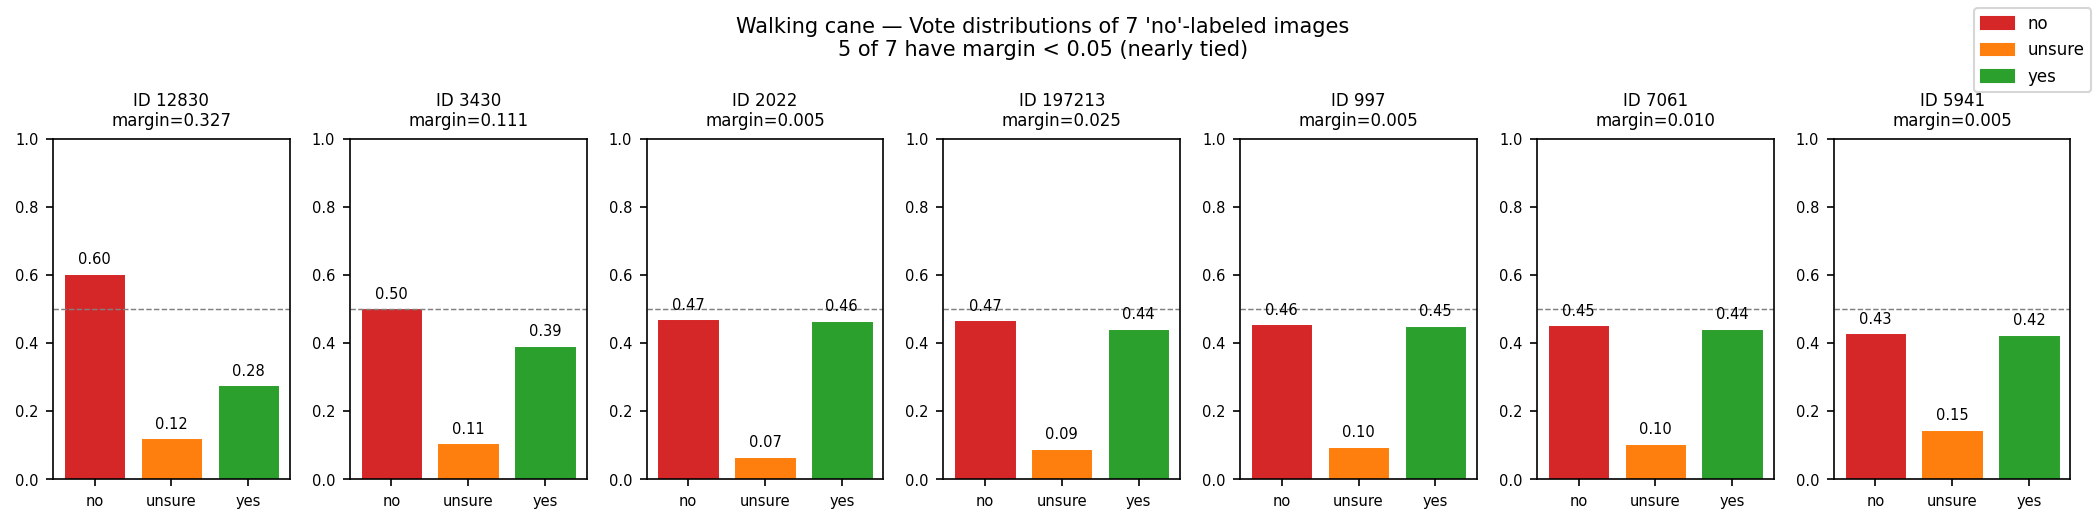
\includegraphics[width=\linewidth]{images/walking_cane_votes.png}
\caption{Vote distributions for the seven majority-``no'' walking-cane images. Five of seven have margin $<0.05$ between top two classes, nearly 50/50 splits that Hard-CE must coerce into hard negatives. Soft-KL preserves the empirical bimodality, explaining the $+42\%$ relative F1 gain in \S\ref{sec:cane}.}
\label{fig:cane_votes}
\end{figure}

\FloatBarrier
\section{Accessibility-Aware Routing}
\label{sec:routing}

Calibrated per-aid probabilities are most useful when embedded in a routing system that can trade accessibility against path length. We demonstrate this on a fixed pedestrian graph of Pittsburgh PA. This experiment should be read as a planner-facing offline evaluation: the graph prior answers which curbside candidates lead to lower-risk pedestrian routes, while a deployed AV would still verify the immediate curbside scene with onboard sensors before opening the door.

\textbf{Graph and edge scoring.} We extract a pedestrian OSM graph of 2,046 nodes and 2,618 undirected edge records fixed to a single GraphML snapshot for reproducibility. 40.4\% of edges are matched directly to Project Sidewalk GPS labels; an additional 51.3\% are scored by querying the nearest labelled Google Street View panorama and running DINOv2-large Soft-KL inference, yielding \textbf{91.7\% label-or-image edge-scoring coverage}. The remaining 8.3\% use population-level priors. The inferred GSV scores are not a constant prior: across all graph edges, mean $\hat{p}_\mathrm{yes}$ ranges from 0.479 for manual wheelchair to 0.668 for walking cane, with 49.5\% of manual-wheelchair edges below 0.5. This distributional spread is what creates useful routing gradients. For comparison, using PS labels alone (40.4\% coverage) produces Brier = 0.010 improvement for walking cane; the 91.7\% label-or-image coverage yields +0.155 (15.5$\times$ larger), because the fixed prior ($\hat{p}_\mathrm{yes} = 0.75$ for cane) was overly optimistic. GSV inference reveals many edges with $\hat{p}_\mathrm{yes} \approx 0.40$ to $0.55$ that the model correctly avoids.

\textbf{Routing objective.} For aid $a$, the edge weight is $\ell_e \cdot (1 + \beta_c\,(1 - \hat{p}^a_{\mathrm{yes},e}))$, where $\ell_e$ is the physical edge length and $\beta_c=8$ is chosen at the inflection of the accessibility-distance Pareto curve. A Monte Carlo sweep over $\beta_c \in \{1, 2, 4, 8, 16\}$ shows the expected accessibility--distance trade-off: mean $\Delta\bar{p}_\mathrm{yes}$ rises from 0.058 to 0.105, while mean distance overhead rises from 2.0\% to 11.3\% (Supplementary). We use $\beta_c=8$ because it achieves most of the accessibility gain (0.097 mean $\Delta\bar{p}_\mathrm{yes}$) before the curve begins to saturate.

\textbf{Canonical OD pair.} Table~\ref{tab:routing} reports per-aid results for a curated origin-destination pair in the Forbes/Murray corridor. Accessibility-weighted routing trades 18 to 25\% extra distance for $+0.134$ to $+0.155$ mean $\hat{p}_\mathrm{yes}$, and each aid selects a \emph{genuinely different} optimal path. This is only possible when real per-edge per-aid scores are available rather than a single binary ``accessible'' flag. Figure~\ref{fig:routes} visualises the five per-aid paths overlaid on the Pittsburgh street network, with the geodesic baseline shown in black. Figure~\ref{fig:routing_summary} summarises accessibility scores and route distances per aid.

\begin{figure}[!t]
\centering
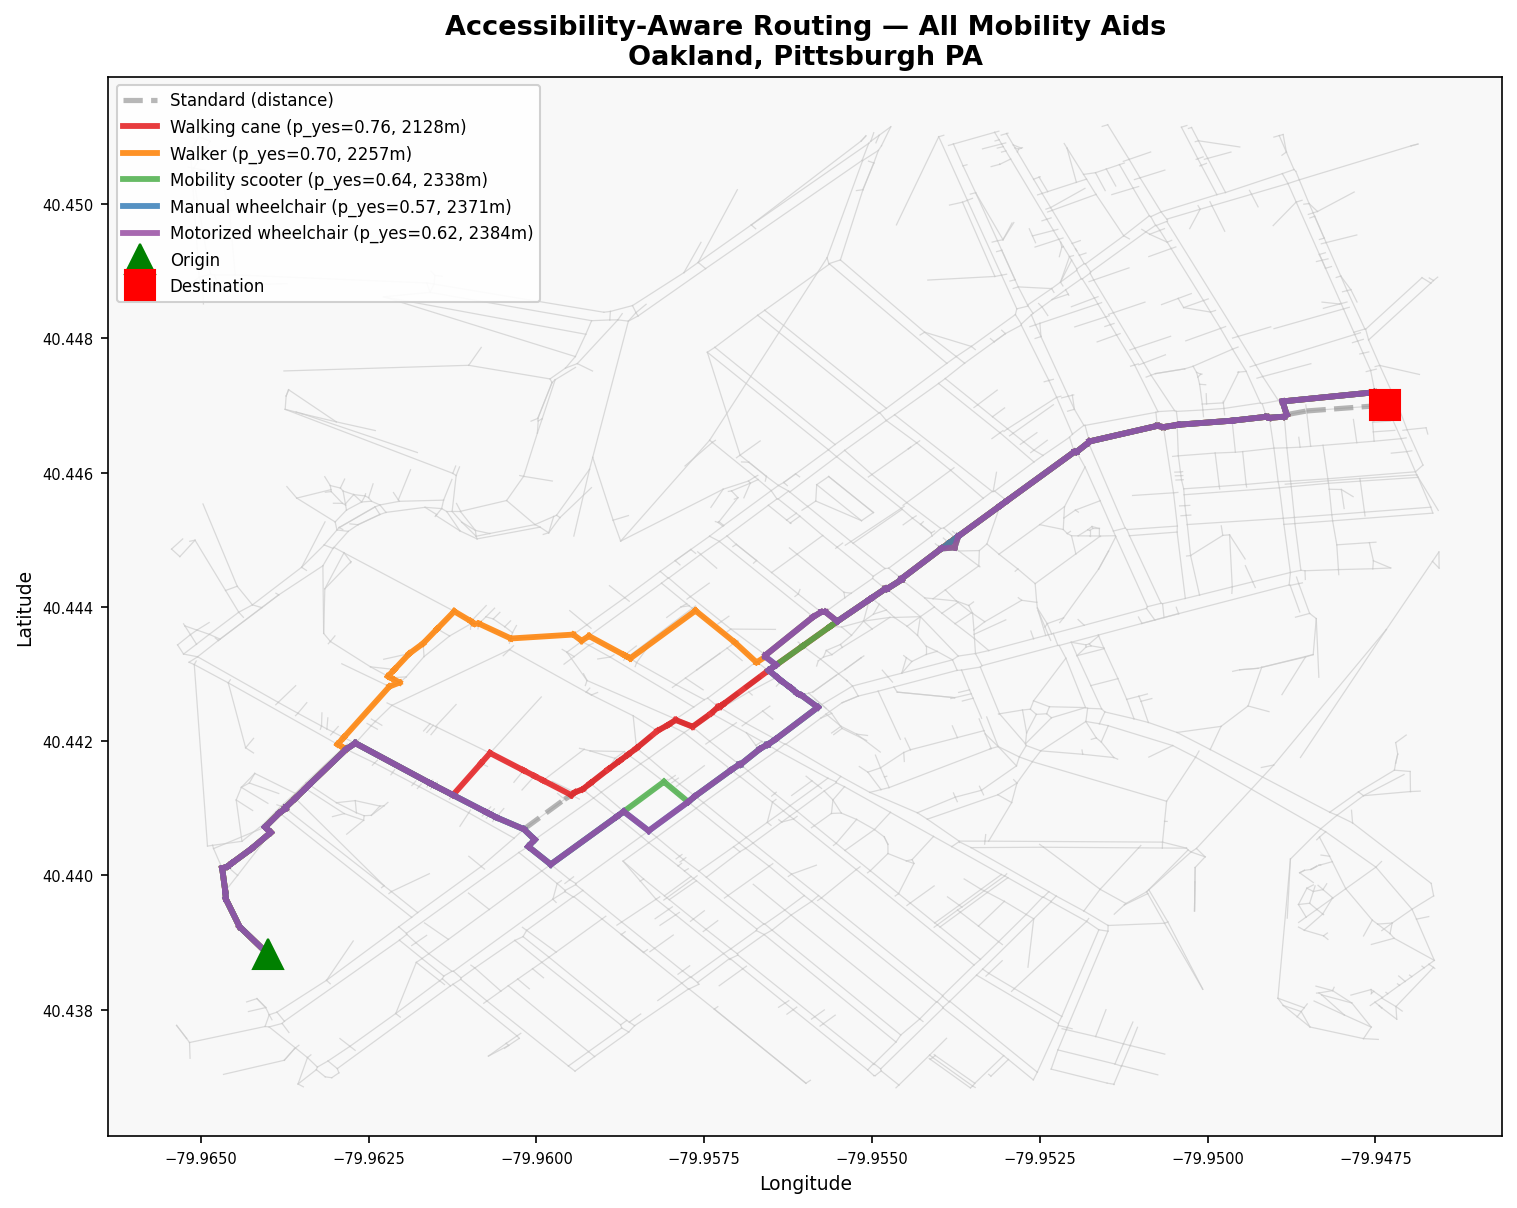
\includegraphics[width=\linewidth]{images/route_all_aids_overlay.png}
\caption{Accessibility-aware routes overlaid on the Pittsburgh OSM pedestrian graph for a single OD pair (green triangle $\to$ red square). Each aid traces a structurally different optimal path under $\beta_c=8$: walking-cane (orange) follows the high-accessibility Forbes corridor; manual wheelchair (purple) detours further north onto smoother sidewalks; the standard shortest path (black) ignores accessibility entirely. Per-aid mean $\hat{p}_\mathrm{yes}$ and total length shown in the legend.}
\label{fig:routes}
\end{figure}

\begin{figure}[!t]
\centering
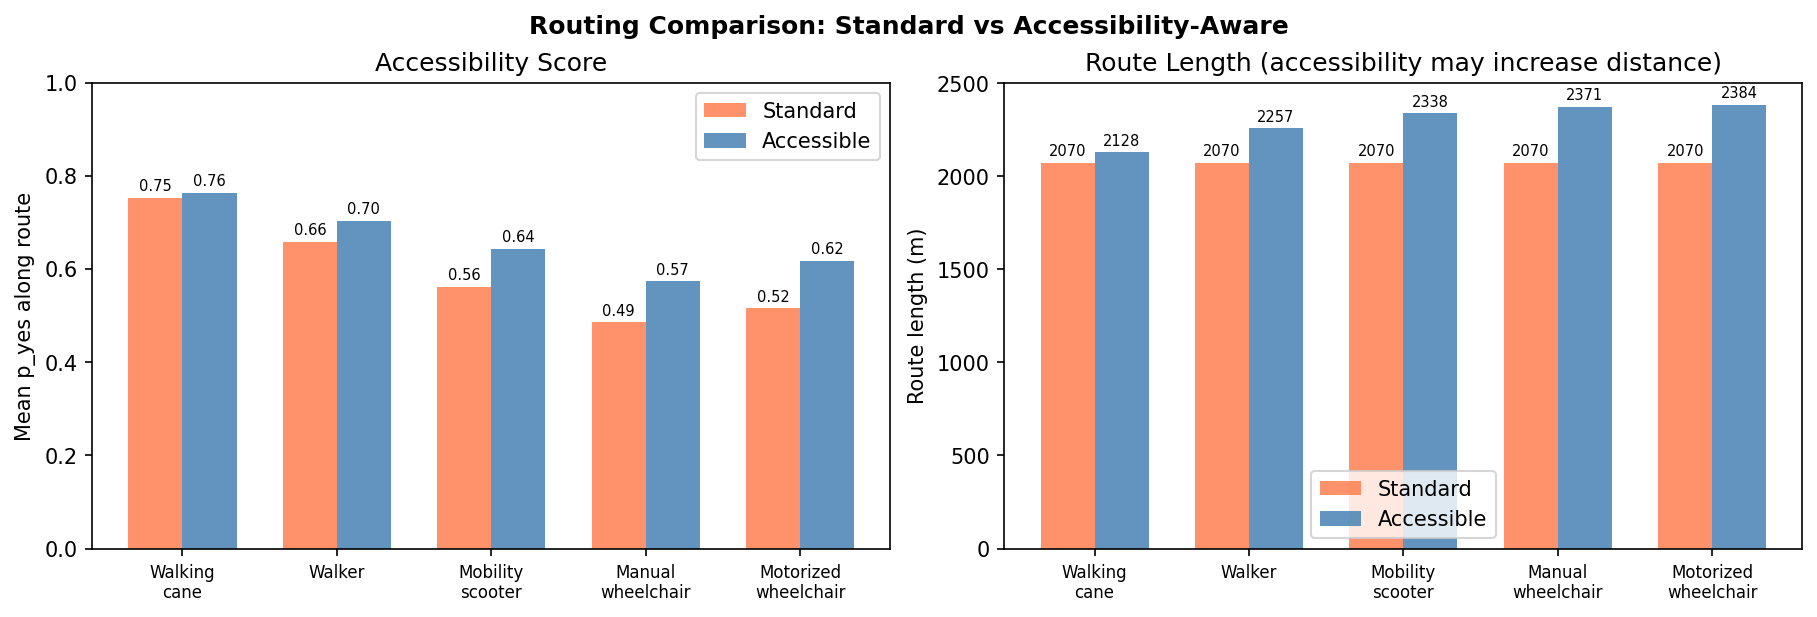
\includegraphics[width=\linewidth]{images/routing_summary.png}
\caption{Per-aid summary for the canonical OD pair: accessibility score (left) and total route length (right). Walking cane (already 0.75 baseline) gains the least in absolute $\hat{p}_\mathrm{yes}$ ($+0.01$) but the most in routing stability; the wheelchair aids gain $+0.07$ to $+0.13$ at $+12$ to $+18\%$ distance.}
\label{fig:routing_summary}
\end{figure}

\begin{table}[!t]
\caption{Accessibility-weighted routing vs.\ standard shortest path, Pittsburgh PA ($\beta_c = 8$, 91.7\% label-or-image edge-scoring coverage). Each aid finds a different optimal route.}
\label{tab:routing}
\centering\small
\setlength{\tabcolsep}{4pt}
\resizebox{\columnwidth}{!}{%
\begin{tabular}{@{}lcccc@{}}
\toprule
\textbf{Mobility Aid} & $\bar{p}^{\mathrm{std}}_{\mathrm{yes}}$ & $\bar{p}^{\mathrm{acc}}_{\mathrm{yes}}$ & $\Delta p_\mathrm{yes}$ & $\Delta\ell$ \\
\midrule
Walking cane         & 0.516 & 0.671 & +0.155 & +575 m (+25\%) \\
Walker               & 0.486 & 0.630 & +0.144 & +575 m (+25\%) \\
Mobility scooter     & 0.459 & 0.600 & +0.141 & +412 m (+18\%) \\
Manual wheelchair    & 0.442 & 0.576 & +0.134 & +447 m (+19\%) \\
Motorized wheelchair & 0.446 & 0.592 & +0.146 & +575 m (+25\%) \\
\bottomrule
\end{tabular}%
}
\end{table}

\textbf{Comparison with ORS wheelchair profile.} OpenRouteService (ORS)~\cite{openrouteservice2026wheelchair} is a widely-used open-source accessible routing engine that uses OSM wheelchair tags (surface, kerb, slope) as edge costs; it is the natural rule-based counterpart to learned alternatives like AccessMap~\cite{bolten2017accessmap,bolten2019opensidewalks} and MyPath~\cite{saha2022mypath}. We compare ORS against our method on 50 random OD pairs in our Pittsburgh graph; we emphasise that this is a single-city, $n=50$ snapshot, not a global benchmark, and the comparison is best read as directional evidence. ORS returns no route for 20\% of pairs due to insufficient OSM wheelchair tags, a coverage failure mode previously documented by Tannert and Sch{\"o}ning~\cite{tannert2018wheelchair}. On the 40 ORS-routable pairs, our method yields a higher mean $\hat{p}_\mathrm{yes}$ on every aid in our Pittsburgh evaluation (Table~\ref{tab:ors}); the paired difference's 95\% CI is positive for all five aids though the lower bound is small ($+0.012$--$+0.025$). The plausible mechanism is coverage: our DINOv2-large + GSV scoring populates $91.7\%$ of edges with a calibrated per-aid probability, while ORS relies on OSM tags that are often missing.

\begin{table}[!t]
\caption{\textbf{ORS wheelchair profile vs.\ our method on 50 Pittsburgh OD pairs.} ORS fails on 20\% of pairs (sparse OSM kerb tags). Mean $\hat{p}_\mathrm{yes}$ on the 40 routable pairs; \textbf{$\Delta$ (Ours--ORS)} is the paired difference with its 95\% CI. The signed difference is positive for every aid in this Pittsburgh snapshot, although the CIs are wide given $n=40$.}
\label{tab:ors}
\centering\small
\setlength{\tabcolsep}{3.5pt}
\resizebox{\columnwidth}{!}{%
\begin{tabular}{@{}lccccc@{}}
\toprule
\textbf{Aid} & \textbf{Std.} & \textbf{ORS} & \textbf{Ours} & \textbf{$\Delta$ (Ours--ORS)} & \textbf{ORS fail} \\
\midrule
Walking cane         & 0.704 & 0.712 & \textbf{0.748} & $+0.036\pm0.018$ & 20\% \\
Walker               & 0.623 & 0.634 & \textbf{0.668} & $+0.034\pm0.020$ & 20\% \\
Mobility scooter     & 0.573 & 0.585 & \textbf{0.625} & $+0.040\pm0.019$ & 20\% \\
Manual wheelchair    & 0.505 & 0.519 & \textbf{0.566} & $+0.047\pm0.022$ & 20\% \\
Motorized wheelchair & 0.532 & 0.545 & \textbf{0.590} & $+0.045\pm0.022$ & 20\% \\
\bottomrule
\end{tabular}%
}
\end{table}

\textbf{Routing failure under miscalibration.} To show concretely that calibration affects route selection, we run an identical routing experiment using Hard-CE DINOv2-large predictions as edge weights. Hard-CE selects a \emph{structurally different} path from Soft-KL for all five aids on the canonical OD pair. When both routes are re-evaluated by the calibrated Soft-KL $\hat{p}_\mathrm{yes}$ metric (Figure~\ref{fig:hardce_comparison}), the Hard-CE route is consistently lower-scoring: gaps range from $+0.013$ (mobility scooter) to $+0.030$ (walker) in mean $\hat{p}_\mathrm{yes}$ per edge. Hard-CE also overestimates its own route quality by $+0.055$ to $+0.085$ per aid because its overconfident predictions report near-1 probabilities for borderline edges, making its self-assessed route score look competitive with Soft-KL's calibrated score. The walker result is representative: Hard-CE claims its route achieves $\hat{p}_\mathrm{yes}=0.684$ but the calibrated evaluation gives $0.600$, an overestimate of $+0.085$ that would cause a risk-aware planner to prefer a lower-scoring path.

\begin{figure}[!t]
\centering
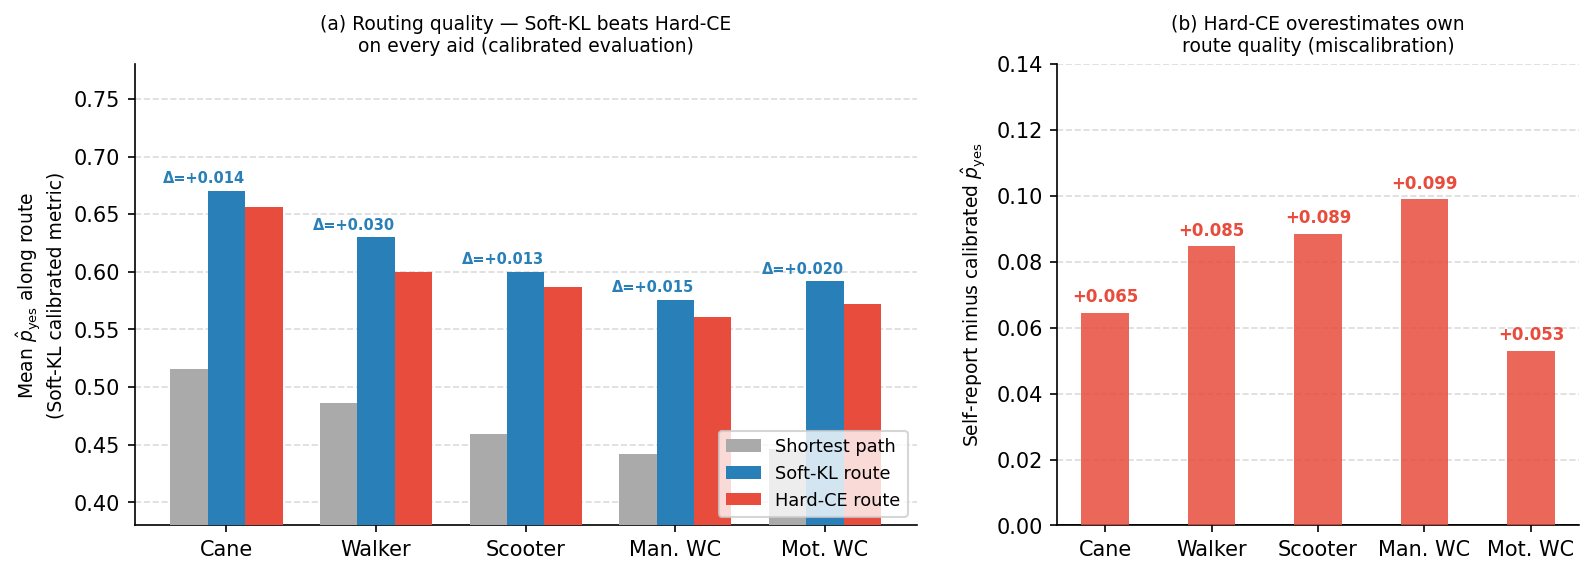
\includegraphics[width=\linewidth]{images/routing_hardce_comparison.png}
\caption{Cross-evaluation of routing under Soft-KL vs Hard-CE edge scores on the canonical Pittsburgh OD pair. Bars show mean $\hat{p}_\mathrm{yes}$ along each route, evaluated by the calibrated Soft-KL metric (our reference risk estimate). Hard-CE routes (solid red) are consistently lower than Soft-KL routes (blue) on the calibrated metric, despite Hard-CE's own inflated self-report (hatched red) appearing higher.}
\label{fig:hardce_comparison}
\end{figure}

\textbf{Monte Carlo evaluation (10,000 OD pairs).} To verify that the canonical route is not a cherry-picked example, we sample 10,000 random origin-destination pairs with a minimum 200 m straight-line separation and compare standard vs.\ accessibility-weighted Dijkstra for all five aids. Table~\ref{tab:montecarlo} reports the results. Across all aids, \textbf{87.8 to 91.0\%} of random Pittsburgh trips yield higher mean $\hat{p}_\mathrm{yes}$ under accessibility-weighted routing at a mean distance overhead of \textbf{7.4 to 9.8\%}. The median overhead (4.8 to 6.8\%) is lower than the mean, indicating that the distribution is mildly right-skewed. Figure~\ref{fig:mc_pareto} shows the Pareto scatter per aid.

\begin{table}[!t]
\caption{\textbf{Monte Carlo routing: 10{,}000 random OD pairs in Pittsburgh.} $\beta_c = 8$, seed = 42, min separation 200~m. \% improved = fraction where the accessible route has higher mean $\hat{p}_\mathrm{yes}$; $\pm$ is the 95\% Wilson CI on the binomial proportion ($n=10{,}000$). Median is well below mean for $\Delta\ell$, indicating that most trips re-route at negligible distance cost.}
\label{tab:montecarlo}
\centering\small
\setlength{\tabcolsep}{3.5pt}
\resizebox{\columnwidth}{!}{%
\begin{tabular}{@{}lcccc@{}}
\toprule
\textbf{Aid} & \textbf{Mean} $\Delta\bar{p}_\mathrm{yes}$ & \textbf{Median} & \textbf{\% improved} & \textbf{Mean} $\Delta\ell$ (\%) \\
\midrule
Walking cane         & +0.065 & +0.055 & $87.8\pm0.6$ & +7.4 \\
Walker               & +0.081 & +0.074 & $88.2\pm0.6$ & +8.2 \\
Mobility scooter     & +0.102 & +0.096 & $91.0\pm0.6$ & +8.6 \\
Manual wheelchair    & +0.120 & +0.112 & $90.9\pm0.6$ & +9.8 \\
Motorized wheelchair & +0.116 & +0.110 & $90.8\pm0.6$ & +9.8 \\
\bottomrule
\end{tabular}%
}
\end{table}

\begin{figure}[!t]
\centering
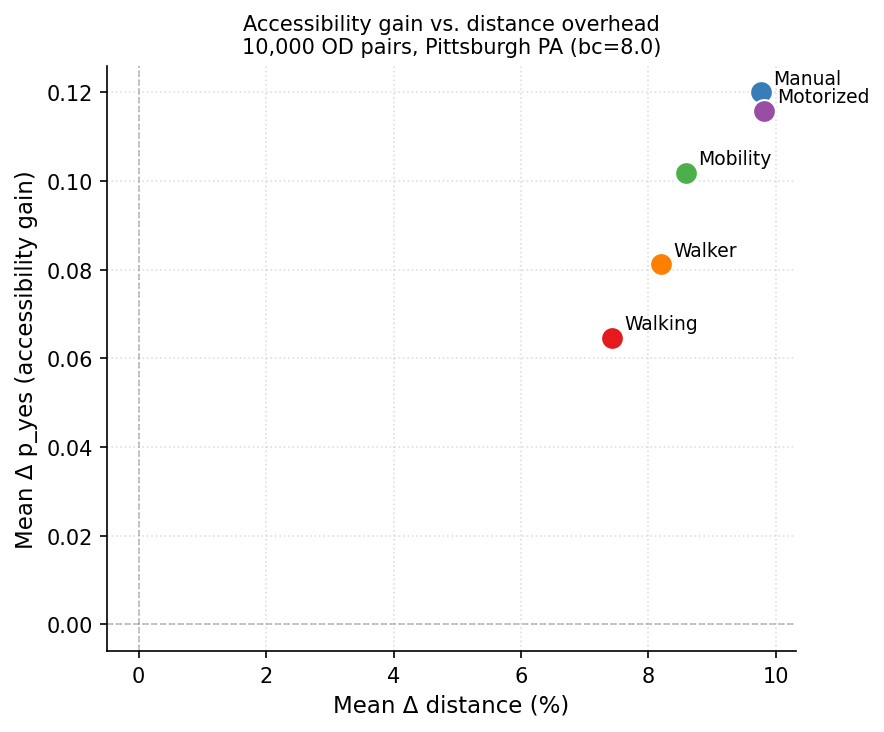
\includegraphics[width=\linewidth]{images/monte_carlo_pareto.png}
\caption{Pareto scatter: mean accessibility gain ($\Delta\bar{p}_\mathrm{yes}$) vs.\ mean distance overhead across 10,000 random OD pairs. All five aids achieve positive accessibility gain at 7 to 10\% extra distance, confirming the routing benefit extends well beyond curated examples.}
\label{fig:mc_pareto}
\end{figure}

\FloatBarrier
\section{Discussion}
\label{sec:discussion}

\textbf{Why DINOv2 without language pretraining?} The near-tie between DINOv2-large and CLIP B/32 at the top of Table~\ref{tab:main} is informative. Traversability perception is not primarily a semantic recognition task. It requires detecting subtle geometric properties: slope, crack width, surface continuity, obstacle clearance. DINOv2's self-supervised training on dense patch-level prediction objectives builds exactly these spatial representations. CLIP's language alignment provides semantic surface-type priors that are partially relevant but come at the cost of weaker local geometry representations. SigLIP2's underperformance relative to its top-ranking results on standard vision-language benchmarks further supports this reading: richer semantic alignment does not transfer to the traversability judgment, where spatial grounding dominates. The ranking inversion between Soft-KL and Hard-CE (DINOv2-large leads Soft-KL, CLIP-B/32 leads Hard-CE) further suggests that DINOv2 features better capture the uncertainty structure of human judgments, while CLIP features better predict the argmax majority class.

\textbf{Calibration is the right metric for routing.} Section~\ref{sec:routing} demonstrates concretely why calibrated probabilities matter. The accessibility-weighted Dijkstra objective treats $\hat{p}_\mathrm{yes}$ as a continuous risk signal: an edge with $\hat{p}_\mathrm{yes}=0.55$ incurs $4\times$ the accessibility penalty of one with $\hat{p}_\mathrm{yes}=0.91$ ($\beta_c=8$). The practical consequence of miscalibration can be quantified directly from Table~\ref{tab:calibration_headline}. Hard-CE (Brier = 0.253, $3.4\times$ the Soft-KL score) places probability mass close to 0 or 1 regardless of underlying human agreement~\cite{guo2017calibration,minderer2021revisiting}: a borderline edge where only 62\% of users voted yes receives $\hat{p}_\mathrm{yes}\approx 0.97$ under Hard-CE (routing penalty $\beta_c(1-\hat{p}) = 0.24$), but $\hat{p}_\mathrm{yes}\approx 0.65$ under Soft-KL (penalty $= 2.8$). The planner's contrast signal for that edge collapses by $12\times$. Applied across the 91.7\% of Pittsburgh edges scored from labels or image inference, this gradient flattens Hard-CE routing toward standard Dijkstra (distance-only): the system can no longer distinguish a 62\%-passable edge from a 97\%-passable one, treating them both as near-safe. Soft-KL's $3\times$ lower Brier score is not a calibration trophy; it is precisely the property that preserves this gradient and enables 88--91\% of random Pittsburgh trips to be meaningfully rerouted at 7--10\% extra distance (Table~\ref{tab:montecarlo}). The ORS comparison reinforces this: ORS's rule-based scoring using sparse OSM tags fails on 20\% of pairs, while our probability-based approach scores all evaluated pairs and yields higher mean $\hat{p}_\mathrm{yes}$ in this snapshot. The result aligns with calibration-aware deployment recommendations for embodied agents~\cite{zollo2025calibration}.

\textbf{Why hard-label ECE can disagree with soft Brier.} Supplementary Table~S5 reports ECE against the majority hard label because that is the standard classification diagnostic. It is not the operational calibration target in this paper. On high-disagreement images, Soft-KL may assign substantial probability mass to ``unsure'' or to the minority class; hard-label ECE counts this as under-confidence if the argmax still matches the plurality label. Hard-CE can therefore obtain lower ECE in some cells by being confidently aligned with the majority class, while still misrepresenting the full human distribution and producing a much worse soft Brier score. Because the planner consumes probability magnitude, not only rank, we treat soft Brier against the full vote distribution as primary and hard-label ECE as secondary.

\textbf{VLMs: competitive F1, poor calibration.} Qwen3-VL-8B comes within 0.041 F1 of our best probe but with Brier 6.2$\times$ worse and 102$\times$ higher latency. The critical failure is calibration: overconfident binary predictions collapse the routing gradient and make VLMs unusable as edge-cost sources even when argmax accuracy is high. Fine-tuning on our 260 soft-label pairs via the KL-divergence objective of Eq.~\ref{eq:softkl} is the most direct path to closing both gaps; the small training-set regime is precisely where Xia et al.~\cite{xia2025softlabels} showed soft-label training provides the largest gain.

\section{Limitations}
\label{sec:limitations}

\textbf{Visual sample size.} The training and cross-validation set is 52 deprojected GSV views from ten cities. This is small by object-recognition standards. We mitigate by using a frozen encoder + linear probe (3075 parameters per aid for DINOv2-large) and by reporting 95\% CIs throughout; the calibration claim does not depend on the absolute F1 value but on the Brier ratio between objectives. Nevertheless, the probe is not expected to extrapolate to arbitrary urban scenes without further data, and the encoder rankings within their overlapping CIs should be read as suggestive, not definitive.

\textbf{Geographic and demographic coverage.} The 52 training views span ten cities, predominantly North-American and European; the auxiliary transfer probe shows Taipei is near chance ($+1.8$pp above the majority-class baseline). The Western-centric data distribution is the headline geographic limitation. Participant demographics beyond mobility-aid type were not collected, so subgroup analysis by age, injury type, or equipment model is not possible. The five mobility-aid categories also conflate equipment heterogeneity (e.g., manual wheelchairs span a wide range of wheel diameters and frame stiffness) that we cannot disaggregate.

\textbf{Single routing city, single graph.} The accessibility-weighted Dijkstra evaluation is on one Pittsburgh OSM graph at one snapshot. We report 95\% Wilson CIs on the binomial improvement rate but cannot characterise routing behaviour under live map updates, in car-sparse rural settings, or in cities with very different morphology. The ORS comparison is $n=50$ pairs in this same graph and should be read as directional evidence, not a global benchmark; the per-aid paired-difference CIs (Table~\ref{tab:ors}) are wide.

\textbf{Offline planner evaluation.} All routing numbers are computed offline on graph edges scored by our probe. This is the appropriate first evaluation for a map-prior layer, but it is not a deployed AV trial. We have not run a live wheelchair-user study, not collected reaction-time data, not measured worst-case route quality under sensor noise or transient obstructions (construction, parked vehicles, snow), and not deployed on a vehicle-embedded compute platform. Latency is measured on a single A100 with sequential inference; behaviour under batched or low-power conditions is unstudied. The closest real-world counterpart to our routing claim is AccessMap~\cite{bolten2017accessmap}; future work should compare in a user study rather than only by mean $\hat{p}_\mathrm{yes}$.

\textbf{Statistical scope.} The 5-fold CV mean F1 differences between Soft-KL and Hard-CE fall within their 95\% CIs for every encoder. We do not claim Soft-KL improves classification accuracy; we claim it improves calibration, where the CI gap is large. The reader should interpret this paper as advocating a metric shift (from argmax to calibrated probability), not as winning the F1 race.

\FloatBarrier
\section{Safety and Responsible Use}
\label{sec:safety}

This system is intended as a perception layer for risk-aware pedestrian routing in autonomous mobility services. We list explicit limits-of-use that, in our view, should accompany any deployment:

\textbf{Not a substitute for human audit.} Our per-aid probability is a community-level prior, not a per-user safety guarantee. The output should inform route ranking, not authorise an AV to commit a wheelchair-user passenger to a particular sidewalk segment without an additional in-loop check (e.g., live sidewalk-sensor verification at drop-off or a passenger-confirmable preview~\cite{saha2022mypath}).

\textbf{Temporal staleness.} GSV imagery is updated on a city-specific cadence (years). Construction sites, temporary obstructions, weather (snow, ice), and recent maintenance are not reflected. A deployed system should compose our static prior with live perception (e.g., onboard LiDAR/camera at curbside) before locking in a route.

\textbf{Personalisation beyond aid type.} The five-class aid taxonomy ignores within-class heterogeneity (chair geometry, motor power, individual risk tolerance). Operationally, $\hat{p}_\mathrm{yes}$ should be exposed to the passenger as an explicit confidence, not a binary decision, and personalised tuning (e.g., a user-specific $\beta_c$ in the routing objective) should be retained.

\textbf{Dual-use of disagreement.} The vote distribution genuinely reflects diverse user opinions; collapsing it back to a label internally would re-introduce exactly the failure mode we set out to fix. Any downstream system that consumes our output should propagate the probability vector, not its argmax.

\textbf{Geographic equity.} Until the Western-centric data limitation (\S\ref{sec:limitations}) is addressed by multi-region data collection, the system should not be deployed as a primary routing engine in regions like East Asia where our auxiliary probe is near chance.

\FloatBarrier
\section{Conclusion}
\label{sec:conclusion}

Sidewalk accessibility assessment is a perception problem that prior work has approached with the wrong objective. Crowdsourced vote distributions from 829 mobility-aid users encode genuine community-level uncertainty that the model should reproduce, not discard through majority-vote collapsing. Training directly against these distributions via KL divergence achieves a soft Brier score of 0.064 to 0.083, roughly 3$\times$ lower than standard cross-entropy, without reducing argmax F1, and this advantage holds consistently across all eight encoders and all five cross-validation folds. The walking cane result is the clearest illustration: Hard-CE collapses below the trivial baseline (F1 = 0.453 vs.\ 0.467) for 6 of 8 encoders because it forces hard labels on genuinely ambiguous human judgments; Soft-KL achieves F1 = 0.640 (+42\%) by preserving the uncertainty structure. Among encoders, DINOv2-large achieves the best calibration-latency trade-off at 78.5\,ms/image, a result driven by dense self-supervised spatial features rather than language alignment. On a binary curb-ramp transfer probe, features trained on the 52-view passability benchmark generalize to Detroit, Zurich, and Taipei (balanced accuracy 0.518 to 0.616); Taipei's near-chance result transparently identifies the limit of Western-centric training data. On Pittsburgh routing, our accessibility-weighted Dijkstra improves mean $\hat{p}_\mathrm{yes}$ by $+0.065$ to $+0.120$ on 87.8--91.0\% of 10,000 random OD pairs at 7.4--9.8\% extra distance, and yields higher mean $\hat{p}_\mathrm{yes}$ than OpenRouteService's wheelchair profile on all five aids in our Pittsburgh $n=50$ snapshot, while routing 20\% more pairs that ORS cannot handle due to absent OSM tags. Modern zero-shot VLMs reach within 0.041 F1 of the best trained probe but at 102$\times$ higher latency and 6.2$\times$ worse Brier score; fine-tuning them on our soft-label pairs is the most direct path to closing both gaps simultaneously. Code and pre-extracted features will be released upon acceptance.

\bibliographystyle{IEEEtran}
\bibliography{refs}

\end{document}
